\documentclass[14pt,a4paper,oneside]{report}		%lớp văn bản
\usepackage{graphicx}
\graphicspath{{images/}}
\usepackage[utf8]{vietnam}						%gói ngôn ngữ tiếng Việt
%--
\usepackage{titlesec}
\usepackage{fancybox}
\usepackage{amsfonts}
\usepackage{latexsym, amsmath, amsxtra, amssymb, amscd, amsthm}	%gói ký tự toán
\usepackage{indentfirst}
\usepackage{fancyheadings}
\usepackage{color,colortbl}		%gói màu
\usepackage{graphicx}			%gói hình ảnh 
\usepackage{hyperref}			%gói liên kết link
\usepackage[top=3.5cm, bottom=3.0cm, left=3.5cm, right=2cm] {geometry}
\linespread{1.5}
\lhead{\textsl{Hệ động lực chuyển mạch - Nguyễn Lê Hoàng}}
\rhead{\textsl{\today}}
%//================================= Begin dinh nghia cac goi lenh
\renewcommand{\contentsname}{Mục lục}
\renewcommand{\chaptername}{Chương}
\renewcommand\bibname{Tài liệu tham khảo}
\newcommand{\gach}{\backslash}
\newtheorem{theorem}{Định lý}[chapter]
\newtheorem{lemma}[theorem]{Bổ đề}
\newtheorem{proposition}[theorem]{Mệnh đề}
\newtheorem{corollary}[theorem]{Hệ quả}
\theoremstyle{definition}
\newtheorem{define}[theorem]{Định nghĩa}
\newtheorem{example}[theorem]{Ví dụ}

\titleformat*{\section}{\huge\bfseries}
\titleformat*{\subsection}{\LARGE\bfseries}
%==================================// End dinh nghia cac goi lenh
%//================================== Begin make title
\title{{\bf  BÁO CÁO}}
\author{Nguyễn Lê Hoàng}

\date{{\em \today}}

%==================================// End make  title

\begin{document}

\thispagestyle{empty}
\thisfancypage{
\setlength{\fboxsep}{0pt}
\fbox}{} 
\begin{center}
\begin{large}
TRƯỜNG ĐẠI HỌC BÁCH KHOA HÀ NỘI
\end{large} \\
\begin{large}
VIỆN TOÁN ỨNG DỤNG VÀ TIN HỌC
\end{large} \\
\textbf{--------------------  *  ---------------------}\\[2.5cm]

\includegraphics[width=3cm,height=3cm,keepaspectratio]{logo.jpg}\\[2.5cm]
{\fontsize{32pt}{1}\selectfont BÁO CÁO ĐỒ ÁN TỐT NGHIỆP}\\
{\fontsize{15pt}{1}\selectfont Đề tài: }\\[1cm]
\end{center}

\hspace{5cm} Sinh viên thực hiện \hspace{4pt}: \hspace{4pt}
\textbf{\parbox[t]{5cm}{    
Nguyễn Lê Hoàng\\
}}\\[12pt]

\hspace{5cm} Giáo viên hướng dẫn :  \hspace{4pt} \textbf{\parbox[t]{5cm}{    
Ts. Hà Thị Ngọc Yến
}}

\vspace{3cm}
\begin{center}
{\fontsize{16pt}{1}\selectfont HÀ NỘI}\\
{\fontsize{16pt}{1}\selectfont \today}
\end{center}

\pagestyle{fancy}	
\Large												%co chu
\maketitle											%make title
\setlength{\baselineskip}{5truept}		%gian dong cho muc luc
\tableofcontents									%tao muc luc
\newpage
\setlength{\baselineskip}{18truept}	%gian dong cho van ban
%//==========================================Begin noi dung bai==

\chapter*{Lời mở đầu}
Các hệ thống điều khiển chuyển mạch đã thu hút được rất nhiều sự quan tâm từ cộng đồng, các nhà toán học không chỉ vì sự phức tạp vốn có của chúng, mà còn là do tầm quan trọng trong các vấn đề thực tiên với nhiều ứng dụng trong tự nhiên, kỹ thuật và khoa học xã hội. Thực tế, các hệ thống trong tự nhiên, xã hội hay kỹ thuật thường không thể mô tả đơn giản chỉ bằng một mô hình duy nhất, nhiều hệ thống còn biểu thị sự chuyển đổi qua lại giữa nhiều mô hình tùy thuộc vào điều kiện, môi trường khác nhau. Các hệ thống sinh học tự nhiên còn chuyển đổi sao cho thích nghi được với sự thay đổi của môi trường bên ngoài. Nên các hệ chuyển mạch là thực sự cần thiết. Sự chuyển mạch cũng đã được thể hiện thông qua một vài hệ thống trong xã hội. Để cải thiện hiệu suất, sự chuyển mạch đã được sử dụng/khai thác rộng rãi trong nhiều hệ thống kỹ thuật như điện tử, hệ thống điện, kiểm soát giao thông và trong một số ngành khác.\\

Việc nghiên cứu lý thuyết và khảo sát về các hệ thống điều khiển chuyển mạch thực sự là khó khăn do sự đa dạng, phong phú và phức tạp của hệ thống. Việc chuyển mạch khiến cho các hệ thống phức tạp hơn nhiều so với các hệ thống chuẩn ban đầu. Các hệ chuyển mạch cho ta thêm các trạng thái, tính chất mới phức tạp hơn mà các hệ thống gốc ban đầu không có. Từ thiết kế các hệ thống điều khiển, sự chuyển mạch cho ta sự thoải mái, tùy ý hơn trong việc thiết kế các hệ thống điều khiển. Các quy luật chuyển mạch có thể được sử dụng để điều khiển các thống chuyển mạch sao cho đạt được hiệu năng tốt hơn của hệ thống. Điều này giúp ta có thể điều khiển hệ thống đạt được mục đích kiểm soát nhất định.\\

Một mặt, sự chuyển mạch có thể gây ra tính bất ngờ, không đoán trước được thay đổi trong các hệ thống động lực, cấu trúc hệ thống, chẳng hạn như thay đổi đột ngột cấu trúc hệ thống do sự hỏng hóc của một vài bộ phận hay hệ thống con, hoặc là do sự kích hoạt ngẫu nhiên của bất kỳ hệ thống con nào đó. Mặt khác, việc chuyển mạch là để kiểm soát hiệu quả các hệ thống phi tuyến phức tạp, còn được gọi là các hệ thống lai. Trong cả hai trường hợp trên, một yếu tố cần thiết là sự tương tác giữa các hệ thống động lực chuyển mạch liên tục và các hệ thống động lực chuyển mạch rời rạc. Các hệ thống động lực chuyển mạch thường bao gồm các hệ thống con và các tín hiệu chuyển mạch phối hợp chuyển đổi giữa các hệ thống con. Các hệ chuyển mạch với các điều kiện ràng buộc, quy luật chuyển mạch khác nhau sẽ tạo ra các hệ thống vô cùng phong phú, đa dạng và phức tạp.\\

Đồ án này sẽ giới thiệu về hệ thống động lực chuyển mạch và trình bày những điều kiển để một hệ chuyển mạch là ổn định dưới sự chuyển mạch tùy ý. Nội dung đồ án gồm hai chương:

Chương 1: Giới thiệu một số khái niệm cơ bản, một vài ví dụ về hệ thống động lực chuyển mạch và tính ổn định của chúng.

Chương 2: Trình bày về hệ chuyển mạch phi tuyến, hệ chuyển mạch tuyến tính và tính ổn định của hệ chuyển mạch dưới sự chuyển mạch tùy ý thông qua hàm Lyapunov. Trong chương này còn đề cập đến các tiêu chuẩn ổn định đại số của các hệ chuyển mạch tuyến tính rời rạc. Sự ổn định này được đặc trưng bởi bán kính phổ của ma trận.\\

Trong quá trình làm đồ án, em đã nhận được sự giúp đỡ, chỉ bảo tận tình của cô giáo TS Hà Thị Ngọc Yến. Em xin chân thành cảm ơn và bày tỏ lòng kính trọng tới cô, người đã dành nhiều thời gian chỉ bảo, hướng dẫn và giúp đỡ em hoàn thành đồ án này.\\
Tuy nhiên, trong quá trình làm đồ án, mặc dù đã hết sức cố gắng nhưng do trình độ còn hạn chế và thời gian có hạn nên việc nghiên cứu và trình bày không thể tránh khỏi nhầm lẫ và thiếu sót. Em mong nhận được sự giúp đỡ đóng góp của các thầy cô và bạn bè để đồ án được hoàn thiện hơn.\\\\
\textit{Sinh viên}\\
Nguyễn Lê Hoàng

\chapter{Giới thiệu về hệ chuyển mạch}
\section{Khái niệm về hệ động lực chuyển mạch}
Hệ động lực chuyển mạch là một hệ động lực mà việc chuyển đổi trạng thái có vai trò không nhất định trong vận hành cũng như sự ổn định của hệ. Cụ thể hơn, hệ động lực chuyển mạch là hệ ghép hai mức độ, mức thấp được điều khiển bởi tập các trạng thái vận hành, mức cao sử dụng tổ hợp chuyển đổi giữa các trạng thái. Mỗi trạng thái vận hành được mô tả bằng một phương trình vi phân hoặc phương trình sai phân. Hệ động lực chuyển mạch tuân thủ nghiêm ngặt các nguyên tắc cơ bản:
\begin{itemize}
  \item Mỗi thời điểm chỉ có đúng một trạng thái vận hành.
  \item Việc chuyển đổi giữa các trạng thái không diễn ra đột ngột, tùy ý.
\end{itemize}
\begin{example}
Động cơ xe máy số:\\
Đối với các loại xe máy thông thường như (dream, wave,...) ta có hộp số xoay vòng gồm số 0, số 1, số 2, số 3, số 4 tương ứng với các trạng thái vận hành của một hệ chuyển mạch. Khi bắt đầu nổ máy, xe ở số 0. Tại mỗi thời điểm khi đang di chuyển thì xe chỉ có thể chạy trong một trạng thái số $k$ nhất định. Việc chuyển số luôn tuân theo một quy tắc tăng một hoặc giảm một và quay vòng như sau số 0 $\leftrightarrow$ số 1 $\leftrightarrow$ số 2 $\leftrightarrow$ số 3 $\leftrightarrow$ số 4 $\leftrightarrow$ số 0.
\end{example}

Một hệ động lực chuyển mạch được mô tả dưới dạng như sau:
\begin{equation} \label{eq1-1}
x^+(t) = f_\sigma(x(t)),
\end{equation}
trong đó $x(t)\in\mathbb{R}^n$ là trạng thái liên tục, $\sigma$ là trạng thái rời rạc nhận giá trị trong tập $M = \{1,...,m\}$ và $f_k, k\in M$ là trường véc-tơ. $x^+$ là toán tử đạo hàm với thời gian liên tục $t\in\mathbb{R}$ (tức là: $x^+(t)=\frac{d}{dt}x(t)$) và là toán tử dịch chuyển tịnh tiến với thời gian là rời rạc $t\in\mathbb{N}$ (tức là: $x^+(t)=x(t+1)$). Như vậy, không gian trạng thái liên tục là không gian Euclid n chiều và không gian trạng thái rời rạc là tập chỉ số $M$ có hữu hạn phần tử. Thời gian là tập các số thực với thời gian là liên tục hay là tập các số nguyên với thời gian là rời rạc. Dựa vào tính chất liên tục hoặc rời rạc của thời gian mà ta gọi hệ là hệ chuyển mạch liên tục hay hệ chuyển mạch rời rạc. Khi có $m$ hệ động lực con thì ta gọi là hệ chuyển mạch m-trạng thái và với $k\in M$ hệ được mô tả dưới dạng:
\begin{equation} \label{eq1-2}
x^+(t) = f_k(x(t)).
\end{equation}

Trạng thái rời rạc $\sigma$ được gọi là tín hiệu chuyển mạch. Nếu $\sigma(t)=i$ thì ta nói rằng hệ con thứ $i$ được kích hoạt tại thời điểm $t$. Tại mỗi thời điểm có một và chỉ một hệ con được kích hoạt, đảm bảo nguyên tắc của hệ chuyển mạch.\\

Ký hiệu $\mathcal{T}$ là tập thời gian.$\mathcal{T}$ có thể đó là tập số thực $(\mathcal{T} = \mathbb{R})$ hay tập số nguyên $(\mathcal{T} = \mathbb{N})$. Cho một số thực $s$, ký hiệu $\mathcal{T}_s$ là khoảng thời gian tính từ thời điểm $s$, $\mathcal{T}_s=\{t\in\mathcal{T} : t\geq s\}$. Cho hai số thực $t_1$ và $t_2$ với $t_1 < t_2$, khoảng thời gian $[t_1, t_2)$ được hiểu là
$$[t_1, t_2)=\{t\in\mathcal{T}: t\geq t_1, t<t_2\}.$$
Mặt khác, khoảng thời gian còn có thể hiểu là đoạn $t_2 - t_1$ với thời gian liên tục hay là các thời điểm trong $[t_1,t_2)$ với thời gian rời rạc. 

Cho hàm liên tục từng khúc $\chi$ xác định trên khoảng $[t_1,t_2)$ và thời điểm $t \in (t_1,t_2)$ như sau:
$$\chi(t+)=\lim_{s\downarrow t}\chi(s), \chi(t-)=\lim_{s\uparrow t}\chi(s)$$
với thời gian là liên tục và
$$\chi(t+)=\chi(t+1), \chi(t-)=\chi(t-1)$$
với thời gian là rời rạc.

Khi các hệ con (\ref{eq1-2}) được cho trước, dáng điệu của hệ chuyển mạch được quyết định bởi tín hiệu chuyển mạch. Ta sẽ phân biệt quỹ đạo chuyển mạch, tín hiệu chuyển mạch và quy luật chuyển mạch.

Một quỹ đạo chuyển mạch là một hàm liên tục phải, xác định trên một khoảng thời gian hữu hạn, nhận giá trị trong $M$.
Cho trước khoảng thời gian $[t_0,t_f)$ với $-\infty < t_0 < t_f < +\infty$, một quỹ đạo chuyển mạch $p$ xác định trên đoạn đó được ký hiệu là $p_{[t_0,t_f)}$. Với một quỹ đạo chuyển mạch $p_{[t_0,t_f)}$, thời điểm $t\in (t_0,t_f)$ được gọi là thời điểm bước nhảy nếu:
$$\sigma(t-)\neq\sigma(t).$$

Giả sử rằng các thời điểm bước nhảy trong $(t_0, t_f)$ được sắp xếp theo thứ tự $t_1 < t_2 < t_3 < \cdots$, thì dãy $t_0,t_1,t_2\cdots$ được gọi là dãy thời điểm chuyển mạch của $\sigma$ trên $[t_0,t_f)$. Tương tự, dãy các trạng thái rời rạc được sắp thứ tự $\sigma(t_0),\sigma(t_1),\sigma(t_2)\cdots$ được gọi là dãy chỉ số chuyển mạch của $\sigma$ trên $[t_0,t_f)$. Dãy cặp thứ tự:
$$(t_0,i_0),(t_1,i_1),\cdots,(t_s,i_s)$$
với $i_k=\sigma(t_k)$, được gọi là dãy chuyển mạch của $\sigma$ trên $[t_0,t_f)$.\\
Quỹ đạo chuyển mạch được gọi là hoàn toàn xác định nếu có một số hữu hạn thời điểm bước nhảy trên khoảng đó. Tập những quỹ đạo chuyển mạch hoàn toàn xác định trên $[t_0,t_f)$ được ký hiệu là $S_{[t_0,t_f)}$.

Một tín hiệu chuyển mạch là một hàm xác định trên một khoảng thời gian vô hạn, nhận giá trị trong $M$.

Giả sử rằng $\theta$ là một tín hiệu chuyển mạch xác định trên $[t_0,+\infty)$ và $[s_1,s_2)$ là đoạn con có độ dài hữu hạn của $[t_0,+\infty)$ thì quỹ đạo chuyển mạch $p_{[s_1,s_2)}$ được gọi là quỹ đạo con của $\theta$ nếu $p(t)=\theta(t)$ với mọi $t\in[s_1,s_2)$. Khái niệm dãy chỉ số và dãy thời điểm chuyển mạch được định nghĩa một cách tương tự như đối với quỹ đạo chuyển mạch.
Một tín hiệu chuyển mạch được gọi là hoàn toàn xác định nếu tất cả các quỹ đạo con của nó là hoàn toàn xác định. Kí hiệu $\theta_{[t_0,+\infty)}$ là tín hiệu chuyển mạch $\theta$ xác định trên $[t_0,+\infty)$. Tập những tín hiệu chuyển mạch hoàn toàn xác định trên $[t_0,+\infty)$ được ký hiệu bởi $\mathcal{S}_{[t_0,+\infty)}$ hoặc $\mathcal{S}$ khi $t_0=0$.\\

Cho trước một cặp hàm $(x(\cdot),\theta(\cdot))$ trên đoạn $[t_0,t_1)$, trong đó $x:[t_0,t_1)\mapsto\mathbb{R}^n$ là hàm liên tục và $\theta:[t_0,t_1)\mapsto M$ là hàm hằng từng khúc. Cặp $(x(\cdot),\theta(\cdot))$ được gọi là nghiệm của hệ (\ref{eq1-1}) trên $[t_0,t_1)$ nếu với hầu hết $t\in [t_0,t_1)$ ta có:
$$\frac{dx(t)}{dt}=f_{\theta(t)}(x(t)).$$

Hệ chuyển mạch (\ref{eq1-1}) được gọi là hoàn toàn xác định (xác định một cách toàn cục) nếu với bất kỳ $\theta\in\mathcal{S}_{[0,+\infty)}$ và $x_0\in\mathbb{R}^n$, tồn tại duy nhất một hàm liên tục $x$ trên $[0,+\infty)$ với $x(0)=x_0$ sao cho cặp $(x(\cdot),\theta(\cdot))$ là một nghiệm của hệ (\ref{eq1-1}) trên $[0,+\infty)$.\\
Khi mỗi hệ con thỏa mãn điều kiện Lipchitz toàn cục:
$$\limsup_{x_1\neq x_2}\frac{|f_k(x_1)-f_k(x_2)|}{|x_1-x_2|} < +\infty,\quad k\in M,$$
thì hệ chuyển mạch là hoàn toàn xác định. Trong đồ án này, ta luôn giả thiết rằng các hệ con thỏa mãn điều kiện Lipchitz, và do đó tính hoàn toàn xác định của hệ luôn được đảm bảo.

Một quy luật chuyển mạch là một quy tắc chuyển mạch mà sinh ra một quỹ đạo chuyển mạch hoặc một tín hiệu chuyển mạch từ một tập các cấu hình ban đầu. Trong đồ án này, ta chỉ xét những quy luật chuyển mạch có dạng:
\begin{equation} \label{eq1-3}
\sigma(t)=\varphi(t,\sigma(t-),x(t)),
\end{equation} 
trong đó $\varphi$ là hàm hằng từng khúc nhận giá trị trong $M$.\\
Một hàm $x(t)$ được gọi là một quỹ đạo trạng thái (liên tục) của hệ (\ref{eq1-1}) qua quy luật chuyển mạch (\ref{eq1-3}) trên $[t_0,t_1)$ nếu (\ref{eq1-1}) và (\ref{eq1-3}) đúng với hầu hết $t\in[t_0,t_1)$. Tín hiệu chuyển mạch tương ứng $\sigma$ được gọi là sinh bởi quy luật chuyển mạch (\ref{eq1-3}) dọc theo $x(\cdot)$ với trạng thái ban đầu $x_0$ trên $[t_0,t_1)$.

Một quy luật chuyển mạch được gọi là hoàn toàn xác định nếu nó sinh ra một tín hiệu chuyển mạch hoàn toàn xác định với trạng thái ban đầu bất kỳ.

Với hệ chuyển mạch (\ref{eq1-1}), một quy luật chuyển mạch hoàn toàn xác định có thể biểu diễn bởi tập $\{\theta^x:x\in\mathbb{R}^n\}$ trong đó $\theta^x$ là tín hiệu chuyển mạch được hoàn toàn xác định, sinh bởi quy luật chuyển mạch đó với trạng thái ban đầu $x$. Hệ chuyển mạch có nghiệm duy nhất với điều kiện ban đầu bất kỳ nếu cả hệ chuyển mạch và quy luật chuyển mạch hoàn toàn xác định. Để thuận tiên, ta ký hiệu quỹ đạo trạng thái liên tục bởi $\phi(\cdot;t_0,x_0,\sigma)$ hoặc $\phi(\cdot;x_0,\sigma)$ khi $t_0=0$.

\section{Ví dụ về hệ chuyển mạch}
Cho hệ phương trình trong $\mathbb{R}^2$:
$$x^+(t) = 
\begin{cases} 
A_1x(t) \mbox{ nếu } x_2\geq 0, \\ 
A_2x(t) \mbox{ nếu } x_2\leq 0,
\end{cases}
$$
trong đó $x=(x_1,x_2)\in\mathbb{R}^2$, $t\in[0,+\infty)$ và
$$
A_1 = \begin{bmatrix} -0.01 & -0.5 \\ 2 & -0.01 \end{bmatrix} ,\quad 
A_2 = \begin{bmatrix} -0.01 & -2 \\ 0.5 & -0.01 \end{bmatrix} .
$$
Nghiệm của hệ con thứ nhất và thứ hai lần lượt là:
\begin{equation} \label{vd1}
\begin{cases}
x_1 = e^{-0.01t}(A\cos t+B\sin t)\\
x_2 = 2e^{-0.01t}(A\cos t-B\sin t)
\end{cases}
\text{và}\quad
\begin{cases}
x_1 = e^{-0.01t}(A\cos t+B\sin t)\\
x_2 = \frac{1}{2} e^{-0.01t}(A\cos t-B\sin t)
\end{cases}
\end{equation}

Khi đó quỹ đạo của chúng lần lượt là:
$$
x^2_1 + \frac{x_2^2}{4} = e^{-0.02t}(A^2+B^2) \quad\text{và}\quad x^2_1 + 4x_2^2 = e^{-0.02t}(A^2+B^2)
$$
Ta có thể thấy, khi $t$ đủ lớn thì các ellip này co về gốc tọa độ. Nghiệm của hai hệ con cho ta thấy được hai hệ này ổn định. Hình \ref{fig:1} là nghiệm của mỗi hệ con - các ellip đồng dạng thu hẹp dần:
\begin{figure}[h]
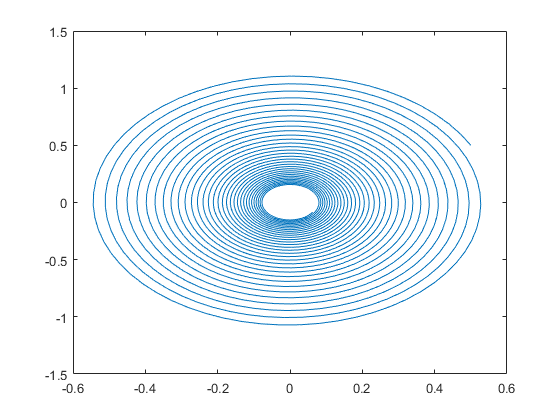
\includegraphics[width=0.5\textwidth]{graph1.png}
\hspace{\fill}
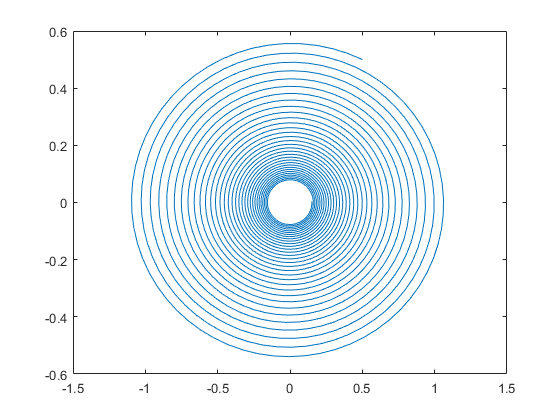
\includegraphics[width=0.5\textwidth]{graph2.png}
\caption{Nghiệm hai hệ con của hệ chuyển mạch $\ref{vd1}$.}\label{fig:1}
\end{figure}
\newpage
Từ đó ta suy ra được nghiệm của hệ chuyển mạch, như hình \ref{fig:2} :
\begin{figure}[h]
\centering
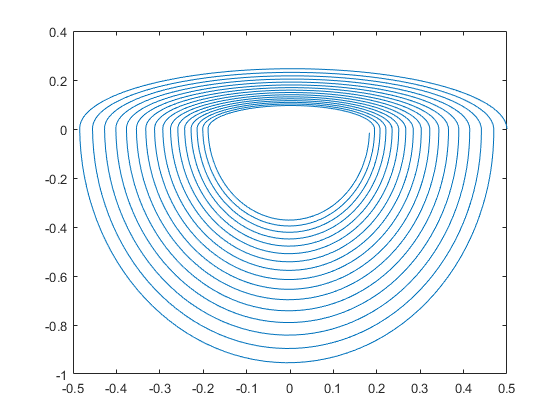
\includegraphics[width=0.5\textwidth]{graph3.png}
\caption{Nghiệm của hệ chuyển mạch $\ref{vd1}$.}\label{fig:2}
\end{figure}\\
Ta có thể thấy rằng, hệ (\ref{vd1}) ổn định. Với quy luật chuyển mạch đã cho như giả thiết thì cứ sau khoảng thời gian $\Delta t=\pi$ thì hệ lại chuyển mạch. Dãy thời điểm chuyển mạch: $\{k\pi | k\in\mathbb{N}\}$. Ta lại xét hệ (\ref{vd1}) nhưng với quy luật chuyển khác như sau: cứ sau khoảng thời gian $\Delta t=2$ thì hệ tự chuyển mạch. Dãy thời điểm chuyển mạch mới: $\{2k|k\in\mathbb{N}\}$. Nghiệm của hệ mới được biểu diễn như hình \ref{fig:3}.
\begin{figure}[h]
\centering
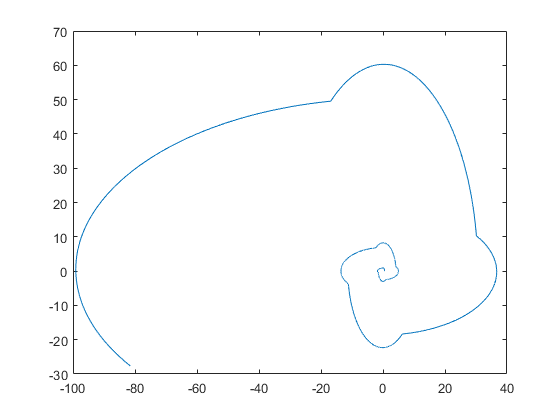
\includegraphics[width=0.5\textwidth]{graph10.png}
\caption{Nghiệm của hệ chuyển mạch $\ref{vd1}$ với quy luật chuyển mạch mới.}\label{fig:3}
\end{figure}
\newpage
Hệ mới ta đang xét lại không ổn định.\\

Vậy hợp các hệ ổn định chưa chắc đã ổn định. Nó còn phụ thuộc vào nhiều yếu tố khác nữa. Ta sẽ tìm hiểu thêm ở các phần sau của đồ án.
\section{Tính ổn định và khả ổn định của hệ chuyển mạch}
Trong các hệ thống động lực, các trạng thái chuyển đổi của hệ thống hoàn toàn được quyết định bởi các cơ chế chuyển đổi. Các hệ thống chuyển mạch có thể rất phức tạp và đa dạng thậm chí khi ta xét một hệ thống con đơn giản cố định. Như vậy ta cần xét đến tính ổn định của các hệ thống chuyển mạch theo các cơ chế chuyển đổi khác nhau. Để xét được tính ổn định, ta cần biết được các khái niêm về tính ổn định của hệ động lực chuyển mạch.
Cho $\Upsilon = \{\Lambda^x:x\in\mathbb{R}^n\}$ với $\Lambda^x$ là tập con khác rỗng của $\mathcal{S}$ - tập các tín hiệu chuyển mạch. Tập này được gọi là tập các tín hiệu chuyển chấp nhận được nếu với mỗi trạng thái ban đầu đều được gán với một tập tín hiệu chuyển mạch. Tập này cảm sinh từ một tập chấp nhận được những quỹ đạo trạng thái liên tục $\{\Gamma_x:x\in\mathbb{R}^n\}$, trong đó $\Gamma_x$ là tập các quỹ đạo trạng thái với trạng thái bắt đầu $x$ và tín hiệu chuyển mạch trong $\Lambda^x$ :
$$\Gamma_x = \{\phi(\cdot;0,x,\theta):\theta\in\Lambda^x\}.$$
Hàm thực $\alpha :\mathbb{R}_+ \mapsto \mathbb{R}_+$ được gọi là thuộc lớp $\mathcal{K}$ nếu nó là hàm liên tục, tăng chặt và $\alpha(0)=0$. Hàm $\alpha$ thuộc lớp $\mathcal{K}$ không bị chặn còn được gọi là lớp $\mathcal{K}_\infty$. Hàm $\beta : \mathbb{R}_+ \times \mathbb{R}_+ \mapsto \mathbb{R}_+$ được gọi là thuộc lớp $\mathcal{KL}$ nếu $\beta(\cdot,t)$ thuộc lớp $\mathcal{K}$ với mỗi điểm cố định $t \geq 0$ và $\lim_{t\rightarrow +\infty}\beta(r,t)=0$ với mỗi $r\geq 0$ cố định.

\begin{define} \label{def1-1} (Tính ổn định) Giả sử $\Upsilon = \{\Lambda^x:x\in\mathbb{R}^n\}$ là tập các tín hiệu chuyển mạch chấp nhận được. Hệ chuyển mạch \ref{eq1-1} được gọi là \\
(1) ổn định $\Upsilon$ nếu tồn tại hàm $\zeta$ thuộc lớp $\mathcal{K}$ và một số thực dương $\delta$ sao cho:
$$|\phi(t;0,x_0,\theta)|\leq\zeta(|x_0|)\qquad\forall t \in [0,+\infty ), x_0 \in\mathbf{B}_\delta , \theta \in\Lambda^{x_0}$$
(2) ổn định $\Upsilon$ nếu tồn tại hàm $\xi$ thuộc lớp $\mathcal{KL}$ sao cho:
$$|\phi(t;0,x_0,\theta)|\leq\xi(|x_0|,t)\qquad\forall t \in [0,+\infty ), x_0 \in\mathbb{R}^n , \theta \in\Lambda^{x_0}$$
(3) ổn định mũ $\Upsilon$ nếu tồn tại các số thực dương $\alpha$ và $\beta$ sao cho:
$$|\phi(t;0,x_0,\theta)|\leq \beta e^{-\alpha t}|x_0|\qquad\forall t \in [0,+\infty ), x_0 \in\mathbb{R}^n , \theta \in\Lambda^{x_0}$$
\end{define}

\begin{define} (Tính khả ổn định) Giả sử $\Upsilon = \{\Lambda^x:x\in\mathbb{R}^n\}$ là tập các tín hiệu chuyển mạch chấp nhận được. Hệ chuyển mạch \ref{eq1-1} được gọi là \\
(1) khả ổn định $\Upsilon$ nếu tồn tại hàm $\zeta$ thuộc lớp $\mathcal{K}$ và một số thực dương $\delta$ và luật chuyển $\{\theta^x:x\in\mathbb{R}^n\}$ với $\theta^x\in\Lambda^x$ sao cho
$$|\phi(t;0,x_0,\theta^{x_0})|\leq\zeta(|x_0|)\qquad\forall t \in [0,+\infty ), x_0 \in\mathbf{B}_\delta$$
(2) khả ổn định $\Upsilon$ nếu tồn tại hàm $\xi$ thuộc lớp $\mathcal{KL}$ và luật chuyển $\{\theta^x:x\in\mathbb{R}^n\}$ với $\theta^x\in\Lambda^x$ sao cho
$$|\phi(t;0,x_0,\theta^{x_0})|\leq\xi(|x_0|,t)\qquad\forall t \in [0,+\infty ), x_0 \in\mathbb{R}^n$$
(3) khả ổn định mũ $\Upsilon$ nếu tồn tại số thực dương $\alpha$ và $\beta$ và luật chuyển $\{\theta^x:x\in\mathbb{R}^n\}$ với $\theta^x\in\Lambda^x$ sao cho
$$|\phi(t;0,x_0,\theta^{x_0})|\leq \beta e^{-\alpha t}|x_0|\qquad\forall t \in [0,+\infty ), x_0 \in\mathbb{R}^n$$
\end{define}

Khi các hệ con là cố định, tính chất ổn định được xác định bởi tập chấp nhận được các tín hiệu chuyển mạch. Nếu $\Upsilon_1\subseteq\Upsilon_2$ thì tính ổn định $\Upsilon_2$ kéo theo tính ổn định $\Upsilon_1$ và tính khả ổn định $\Upsilon_1$ kéo theo tính khả ổn định $\Upsilon_2$.

\subsection{Tính ổn định đảm bảo dưới sự chuyển mạch tùy ý}
Khi sự chuyển mạch giữa các hệ con xuất hiện theo cách bất kỳ thì khi đó tính ổn định được gọi là tính ổn định đảm bảo. Tập chấp nhận được các tín hiểu chuyển mạch được cho bởi:

$$\Upsilon_{as}=\{\Lambda^x:x\in\mathbb{R}^n\},\quad \Lambda^x=\mathcal{S},\forall x\in\mathbb{R}^n$$
là tập lớn nhất trong tất cả các tập chấp nhận được các tín hiệu chuyển mạch. Do đó, tính ổn định đảm bảo là khái niệm chặt nhất trong các khái niệm ổn định. Đặc biệt, khi hệ chuyển mạch ổn định đảm bảo sẽ kéo theo tính ổn định của các hệ con. Điều ngược lại không đúng và được chứng minh thông qua ví dụ sau.\\
\begin{example}
Cho hai hệ con tuyến tính phẳng \cite{DATN5}:
$$\dot{x}=A_1x=
\begin{bmatrix}
0 & 1\\
-1 & -1
\end{bmatrix}x$$
và
$$\dot{x}=A_2x=
\begin{bmatrix}
0 & 1\\
-1-3a & -1-a
\end{bmatrix}x,$$
trong đó $a$ là một tham số thực không âm. Cả hai hệ con đều ổn định mũ. Ta có quy luật chuyển mạch giữa hai hệ con như hình $\ref{fig:4}$.\\
\newpage
\begin{figure}[h]
\centering
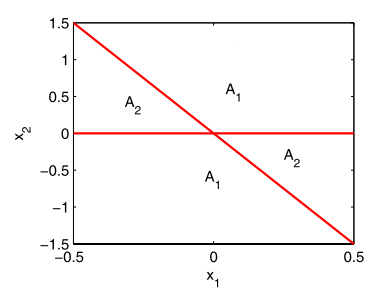
\includegraphics[width=0.5\textwidth]{graph12.png}
\caption{Quy luật chuyển mạch.}\label{fig:4}
\end{figure}
Khi $a=0$ thì hai hệ con trùng nhau nên hệ chuyển mạch là ổn định mũ đảm bảo (Hình \ref{fig:5} với $x_0=[-1/3,1]^T$).
\begin{figure}[h]
\centering
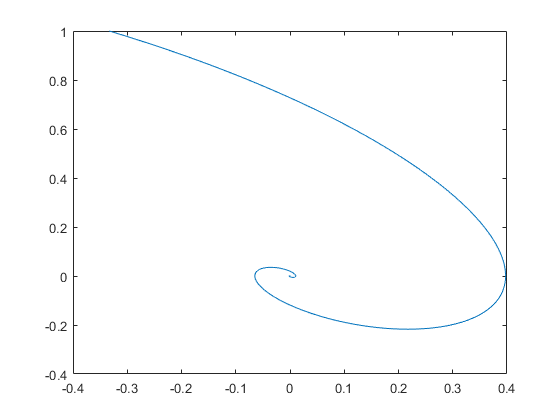
\includegraphics[width=0.5\textwidth]{graph7.png}
\caption{Nghiệm của hệ chuyển mạch khi $a=0$ với $x_0=[-1/3,1]^T$.}\label{fig:5}
\end{figure}

Khi $a=10$ thì hệ chuyển mạch cũng ổn định (Hình \ref{fig:11}).
\begin{figure}[h]
\centering
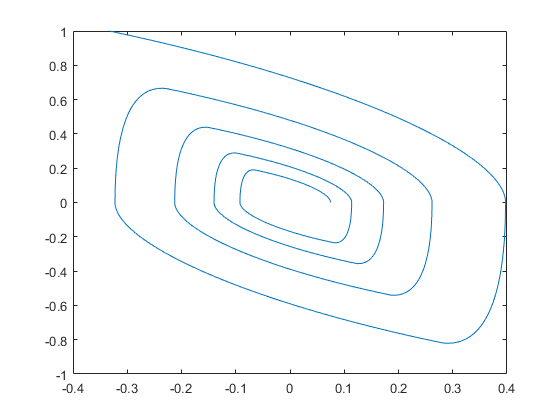
\includegraphics[width=0.5\textwidth]{graph5.png}
\caption{Nghiệm của hệ chuyển mạch khi $a=10$ với $x_0=[-1/3,1]^T$.}\label{fig:11}
\end{figure}
\newpage
Khi $a\approx 36.512$ thì hệ chuyển mạch là ổn định biên đảm bảo (Hình \ref{fig:6}).
\begin{figure}[h]
\centering
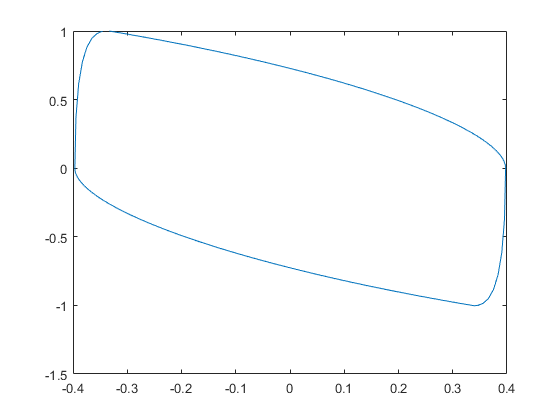
\includegraphics[width=0.5\textwidth]{graph4.png}
\caption{Nghiệm của hệ chuyển mạch khi $a\approx 36.512$ với $x_0=[-1/3,1]^T$.}\label{fig:6}
\end{figure}\\

Khi $a>36.512$ hệ chuyển mạch không ổn định đảm bảo (Hình \ref{fig:7}).
\newpage
\begin{figure}[h]
\centering
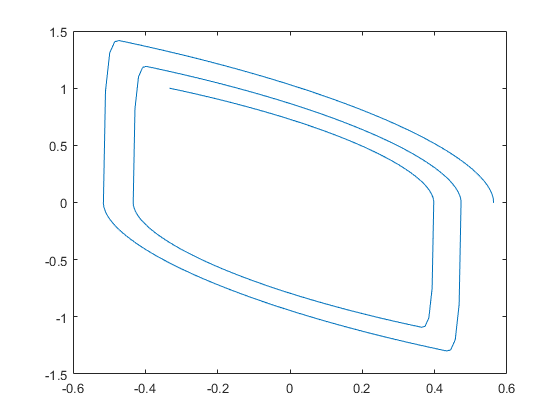
\includegraphics[width=0.5\textwidth]{graph6.png}
\caption{Nghiệm của hệ chuyển mạch khi $a=100$ với $x_0=[-1/3,1]^T$.}\label{fig:7}
\end{figure}
\end{example}

\subsection{Tính ổn định thời gian dừng}
Một tín hiệu chuyển mạch được gọi là thời gian dừng $\tau$ nếu $t_{i+1}-t_i\geq\tau$ với $t_i$ và $t_{i+1}$ là hai thời điểm bước nhảy liên tiếp bất kỳ. Cho $\mathcal{S}_\tau$ là tập tín hiệu chuyển mạch hoàn toàn xác định với thời gian dừng $\tau$. Rõ ràng rằng $\mathcal{S}=\mathcal{S}_0\supseteq\mathcal{S}_{\tau_1}\supseteq\mathcal{S}_{\tau_2}$ với $0\leq\tau_1\leq\tau_2$, và quan hệ tập con là chặt nếu $0<\tau_1<\tau_2$.\\

Tập tín hiệu chuyển mạch $\mathcal{S}$ cho phép sự điều khiển chuyển mạch nhanh một cách tùy ý, thậm chí không có một thời gian dừng đều giữa các thời điểm chuyển mạch.\\

Ví dụ, cho tín hiệu chuyển mạch:

$$\theta(t)=\begin{cases}
1\quad\text{nếu } t\in[k,k+\frac{1}{k+2}), k=0,1,2,\cdots,\\
2\quad\text{các trường hợp khác}
\end{cases}$$
là hoàn toàn xác định, nhưng độ dài của khoảng thời gian chuyển mạch $[k,k+\frac{1}{k+2})$ tiến dần tới $0$ khi $k\rightarrow +\infty$. Rõ ràng những tín hiệu chuyển mạch này thuộc $\mathcal{S}_0$ nhưng nó không thuộc bất kỳ $\mathcal{S}_\tau$ nào với $\tau>0$.\\

Cố định $\tau \geq 0$, cho một tập chấp nhận được các tín hiệu chuyển mạch:
$$\Upsilon_\tau=\{\Lambda^x:x\in\mathbb{R}^n\},\quad \Lambda^x=\mathcal{S}_\tau,\forall x\in\mathbb{R}^n.$$
Tính ổn định của hệ chuyển mạch theo $\Upsilon_\tau$ được gọi là tính ổn định thời gian dừng $\tau$. Một điều kiện cần đối với tính ổn định thời gian dừng $\tau$ là mỗi hệ con đều ổn định. Điều ngược lại đúng cho trường hợp ổn định mũ, tức là nếu các hệ con ổn định mũ thì hệ chuyển mạch ổn định mũ thời gian dừng $\tau$ với $\tau$ đủ lớn. Thật vậy, từ tính ổn định mũ của các hệ con, ta suy ra sự tồn tại của một thời gian $T>0$ sao cho:
$$|\phi_i(t;x_0)|\leq\frac{1}{2}|x_0|\quad\forall t\in\mathcal{T}_T,x_0\in\mathbb{R}^n,$$
trong đó $\phi_i(\cdot;x_0)$ ký hiệu cho quỹ đạo trạng thái của hệ con thứ $i$ với $x(0) = x_0$. Do đó hệ chuyển mạch là ổn định mũ thời gian dừng $\tau$. Tuy nhiên, khẳng định này không đúng cho trường hợp ổn định tiệm cận và ổn định biên.

\begin{example}
Cho hệ chuyển mạch tuyến tính với hai hệ con ổn định biên \cite{DATN5}:
$$\dot{x}=A_1x=
\begin{bmatrix}
0 & 1\\
-2 & -0
\end{bmatrix}x$$
và
$$\dot{x}=A_2x=
\begin{bmatrix}
0 & 1\\
-\frac{1}{2} & 0
\end{bmatrix}x,$$
Ngiệm của hai hệ con (Hình \ref{fig:8}).\\
\begin{figure}[h]
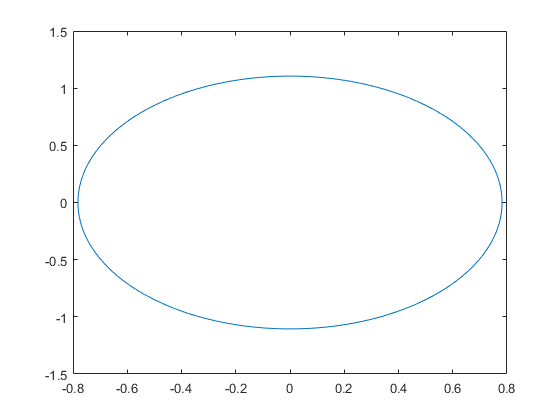
\includegraphics[width=0.5\textwidth]{graph8.png}
\hspace{\fill}
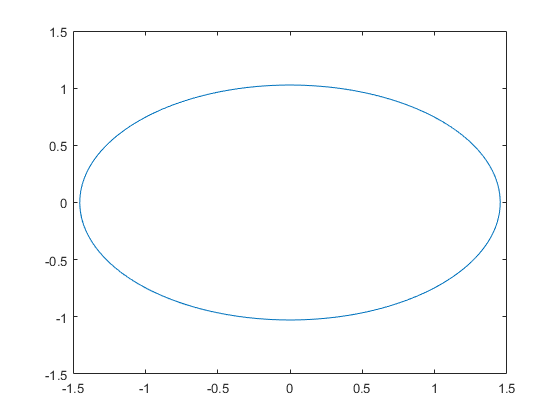
\includegraphics[width=0.5\textwidth]{graph9.png}
\caption{Nghiệm hai hệ con của hệ chuyển mạch.}\label{fig:8}
\end{figure}\\
Ta xét quy luật chuyển mạch dưới đây (\ref{fig:9}).\\
\begin{figure}[h]
\centering
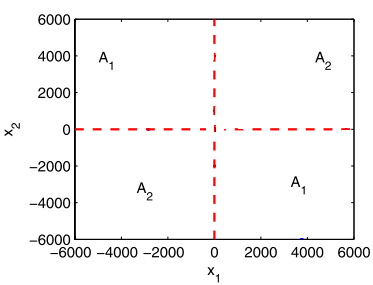
\includegraphics[width=0.5\textwidth]{graph13.png}
\caption{Quy luật chuyển mạch.}\label{fig:9}
\end{figure}
Hệ chuyển mạch sẽ không ổn định. Khi quỹ đạo của mỗi hệ con là tuần hoàn, bằng việc ghép một hoặc nhiều chu kỳ vào mỗi khoảng thời gian chuyển mạch thì trạng thái luôn phân kỳ.\\
\begin{figure}[h]
\centering
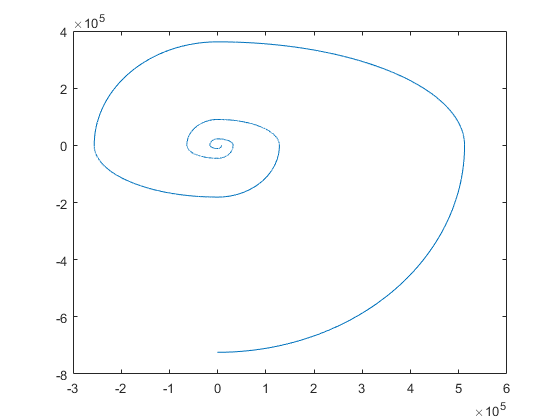
\includegraphics[width=0.5\textwidth]{graph11.png}
\caption{Nghiệm của hệ chuyển mạch.}\label{fig:10}
\end{figure}\\
Từ đó suy ra, với $\tau > 0$ bất kỳ, tập chấp nhận được $\Upsilon_\tau$ chứa những tín hiệu chuyển mạch làm mất tính ổn định. Vậy với tính ổn định thời gian dừng, bài toán đặt ra là phải đi tìm $\tau$ nhỏ nhất sao cho hệ chuyển mạch ổn định.
\end{example}

\chapter{Tính ổn định của hệ chuyển mạch dưới sự chuyển mạch tùy ý}
\section{Một số khái niệm cơ bản}
Trong chương này, ta sử dụng thuật ngữ "ổn đinh đảm bảo" để mô tả tính ổn định của hệ chuyển mạch khi sự chuyển mạch xuất hiện một cách tùy ý.\\

Xét hệ động lực chuyển mạch sau:
\begin{equation} \label{eq2-1}
x^+(t)=f(x(t),\sigma (t)),
\end{equation}
trong đó $x(t)\in\mathbb{R}^n$ là trạng thái liên tục, $\sigma (t)\in M = \{1,...,m\}$ là trạng thái rời rạc và $f : \mathbb{R}^n \times M \mapsto \mathbb{R}^n$ là trường vec-tơ với $f(\cdot ,i)$ là hàm liên tục Lipschitz với mọi $i\in M$.\\\\
Ta định nghĩa hàm $f_i : \mathbb{R}^n \mapsto \mathbb{R}^n$:
$$f_i(x)=f(x,i), \qquad i\in M.$$
Khi đó, hệ \ref{eq2-1} được viết lại dạng
\begin{equation} \label{eq2-2}
x^+(t)=f_{\sigma (t)}(x(t)).
\end{equation}

Trong chương này, ta sẽ đi phân tích tính ổn định của hệ \ref{eq2-2} với vài giả thiết sau:\\
(1) $f_i(0)=0$ với mọi $i\in M$, đó là gốc cân bằng.\\
(2) Hệ liên tục Lipschitz toàn cục, tức là tồn tại hằng số dương $L$ sao cho
\begin{equation} \label{eq2-3}
|f_i(x)-f_i(y)|\leq L|x-y|\qquad \forall x,y \in \mathbb{R}^n,\forall i\in M,
\end{equation}
Giả thiết (1), (2) vừa đưa ra đảm bảo tính đặt chỉnh của hệ thống chuyển mạch.\\
Ta định nghĩa $\phi (t;t_0,x_0,\sigma)$ là trạng thái chuyển liên tục của hệ \ref{eq2-2} tại thời điểm $t$ với điều kiện ban đầu $x(t_0)=x_0$ và cơ chế chuyển $\sigma$. Ta sử dụng $\phi (t;x_0,\sigma)$ là nghiệm tại thời điểm $t_0 = 0$. Với mọi điều kiện ban đầu $x(t_0)=x_0$ và thời điểm $t>t_0$, với thời gian rời rạc ta có

\begin{equation} \label{eq2-4}
\phi (t;t_0,x_0,\sigma)=f_{\sigma (t-1)}\circ \cdots \circ f_{\sigma (t_0+1)}\circ f_{\sigma (t_0)}(x_0),
\end{equation}
trong đó $\circ$ là hàm hợp, $f_1 \circ f_2(x) = f_1(f_2(x))$. Với thời gian là liên tục ta có

\begin{equation} \label{eq2-5}
\phi (t;t_0,x_0,\sigma )=\Phi^{f_{i_s}}_{t-t_s}\circ\Phi^{f_{i_{s-1}}}_{t_s-t_{s-1}}\circ\cdots\circ\Phi^{f_{i_{1}}}_{t_2-t_{1}}\circ\Phi^{f_{i_{0}}}_{t_1-t_{0}}(x_0)
\end{equation}
trong đó $\Phi^f_t(x_0)$ là giá trị của tích phân hàm $f$ đi qua $x(0)=x_0$ và $(t_0,i_0),\cdots ,(t_s,i_s)$ là trình tự chuyển của $\sigma$ trong $[t_0,t)$.\\
Để đưa ra định nghĩa về tính ổn định của hệ chuyển mạch, ta cần thêm một vài định nghĩa sau. Gọi $d(x,y)$ là khoảng cách Euclide giữa $x$ và $y$. Cho tập $\Omega \subset\mathbb{R}^n$ và véc-tơ $x\in\mathbb{R}^n$, đặt $|x|_\Omega = \inf_{y\in\Omega}d(x,y)$. Cho tập $\Omega\subset\mathbb{R}^n$ và một số thực dương $\tau$, gọi $\mathbf{B}(\Omega , \tau)$ là $\tau$-lân cận của $\Omega$ :
$$\mathbf{B}(\Omega,\tau)=\{x\in\mathbb{R}^n:|x|_\Omega\leq\tau\}.$$
Tương tự, gọi $\mathbf{H}(\Omega,\tau)$ là $\tau$-mặt cầu của $\Omega$ :

$$\mathbf{H}(\Omega,\tau)=\{x\in\mathbb{R}^n:|x|_\Omega=\tau\}.$$
Đặc biệt, hình cầu đóng $\mathbf{B}(\{0\},\tau)$ được ký hiệu là $\mathbf{B}_\tau$, và mặt cầu $\mathbf{H}(\{0\},\tau)$ được ký hiệu là $\mathbf{H}_\tau$.

\begin{define} \label{def2-1}
Điểm cân bằng O của hệ \ref{eq2-2} được gọi là\\
(1) điểm hấp dẫn (hút) đảm bảo toàn cục nếu
$$\lim_{t\rightarrow +\infty}|\phi (t;x,\sigma)|=0\qquad\forall x\in\mathbb{R}^n, \sigma\in\mathcal{S}$$
(2) điểm hấp dẫn đảm bảo toàn cục đều nếu với mọi $\delta >0$ và $\epsilon >0$, tồn tại $T>0$ sao cho
$$|\phi (t;x,\sigma)|<\epsilon\qquad\forall t\in\mathcal{T}_T, |x|<\delta,\sigma\in\mathcal{S}$$
(3) điểm ổn định nếu với mọi $\epsilon > 0$ và $\sigma\in\mathcal{S}$, tồn tại $\delta >0$ sao cho
$$|\phi (t;x,\sigma)|<\epsilon\qquad\forall t\in\mathcal{T}_0, |x|<\delta$$
(4) điểm ổn định đều nếu tồn tại $\delta > 0$ và lớp $\mathcal{K}$ hàm $\gamma$ sao cho
$$|\phi (t;x,\sigma)|\leq \gamma(|x|)\qquad\forall t\in\mathcal{T}_0, |x|<\delta,\sigma\in\mathcal{S}$$
(5) điểm ổn định tiệm cận toàn cục nếu nó vừa là điểm ổn định vừa là điểm hấp dẫn đảm bảo toàn cục\\
(6) điểm ổn định tiệm cận đều toàn cục nếu nó vừa là điểm ổn định đều vừa là điểm hấp dẫn đảm bảo toàn cục đều\\
(7) đảm bảo ổn định mũ toàn cục nếu với mọi $\sigma\in\mathcal{S}$, tồn tại $\alpha>0$ và $\beta >0$ sao cho
$$|\phi (t;x,\sigma)|\leq \beta e^{-\alpha t}|x|\qquad\forall t\in\mathcal{T}_0, x\in\mathbb{R}^n$$
(8) điểm ổn định mũ đều toàn cục nếu tồn tại $\alpha>0$ và $\beta >0$ sao cho
$$|\phi (t;x,\sigma)|\leq \beta e^{-\alpha t}|x|\qquad\forall t\in\mathcal{T}_0, x\in\mathbb{R}^n, \sigma\in\mathcal{S}$$
\end{define}

Hệ được đảm bảo ổn đinh/hút nếu gốc cân bằng của nó là đảm bảo ổn định/hút. Từ chương này trở đi để cho gọn các từ "đảm bảo" và "toàn cục" sẽ được loại bỏ. Sự ổn định tiệm cận/mũ thống nhất phù hợp trong định nghĩa \ref{def1-1}.

\section{Hệ chuyển mạch phi tuyến}
Trong phần này, ta sẽ xét vấn đề ổn định của hệ chuyển mạch phi tuyến
\begin{equation} \label{eq2-6}
x^+(t)=f_{\sigma (t)}(x(t))
\end{equation}
dưới sự chuyển mạch bất kỳ.
\subsection{Các hàm Lyapunov thông dụng}
Hàm liên tục $V(x): \mathbb{R}^n\mapsto \mathbb{R}$ với $V(0)=0$ là:\\
(1) xác định dương $(V(x)\succ 0)$ nếu $V(x)>0\forall x\in\mathbb{R}^n-\{0\}$ \\
(2) nửa xác định dương $(V(x)\succeq 0)$ nếu $V(x)\geq 0\forall x\in\mathbb{R}^n$ \\
(3) không bị chặn ngoài nếu tồn tại hàm $\alpha (\cdot)$ thuộc lớp $\mathcal{K}_\infty$ sao cho $V(x)\geq \alpha(|x|)\forall x\in\mathbb{R}^n$ \\

\begin{define} \label{def2-2}
Cho $\Omega$ là lân cận ở của O. Hàm $V:\Omega \mapsto\mathbb{R}$ được gọi là hàm Lyapunov yếu (CWLF) cho hệ chuyển mạch (\ref{eq2-6}) nếu \\
(1) nó là nửa liên tục dưới trên $\Omega$\\
(2) nó nhận hàm $\alpha_1$ và $\alpha_2$ thuộc lớp $\mathcal{K}$ sao cho
$$\alpha_1(|x|)\leq V(x)\leq \alpha_2(|x|)\qquad \forall x\in\Omega$$\\
(3) với mọi $x\in\Omega$ và $i\in M$ ta có
$$\mathcal{D}^+V(x)|_{f_i} = \lim_{\tau \rightarrow 0^+}\sup\frac{V(\phi(\tau;0,x,\widehat{i}))-V(x)}{\tau}\leq 0$$
với thời gian là liên tục, trong đó $\widehat{i}$ là tín hiệu chuyển hằng $\sigma(t)\equiv i\; \forall t,$ và
$$\mathcal{D}^+V(x)|_{f_i}=V(f_i(x))-V(x)\leq 0$$
với thời gian là rời rạc.
\end{define}

\textit{Lưu ý:} Hàm Lyapunov yếu không cần là liên tục. Thực tế, ngay cả một hệ thống phi tuyến ổn định đều $\dot{x}=f(x)$ với $f$ là hàm đủ trơn có thể không nhận hàm Lyapunov yếu nào cả.

\begin{define} \label{def2-4}
Hàm $V:\mathbb{R}^n\mapsto\mathbb{R}$ được gọi là hàm Lyapunov mạnh (CLF) cho hệ chuyển mạch (\ref{eq2-6}) nếu\\
(1) nó liên tục tại mọi điểm và liên tục khả vi trừ điểm gốc\\
(2) nó bị chặn bởi lớp $\mathcal{K}_\infty$, tức là tồn tại hàm $\alpha_1$ và $\alpha_2$ thuộc lớp $\mathcal{K}_\infty$ sao cho
$$\alpha_1(|x|)\leq V(x)\leq \alpha_2(|x|)\qquad\forall x\in\mathbb{R}^n,$$
(3) có hàm $\alpha_3: \mathbb{R}^n\mapsto\mathbb{R}_+$ thuộc lớp $\mathcal{K}$ sao cho
\begin{equation} \label{eq2-7}
\mathcal{D}^+V(x)|_{f_i}\leq -\alpha_3(|x|)\qquad\forall x\in\mathbb{R}^n, i\in M.
\end{equation}
\end{define}
\textit{Chú ý:} Với thời gian là liên tục thì
\begin{equation} \label{eq2-8}
\mathcal{D}^+V(x)|_{f_i}=\limsup_{\tau\rightarrow 0^+}\frac{V(x+f_i(x)\tau)-V(x)}{\tau}\qquad\forall x\in\mathbb{R}^n,i\in M,
\end{equation}
do tính liên tục Lipschitz địa phương của $V$. Cho hàm khả vi liên tục $V$ ta có
$$\mathcal{D}^+V(x)|_f=\frac{d}{dt}V(x)=L_fV(x)=\frac{\partial}{\partial x}V(x)f(x).$$
Trước hết, giả sử hệ (\ref{eq2-6}) chấp nhận một hàm Lyapunov yếu. Với mọi trạng thái $x(t)=\phi(t;x_0,\sigma)$ trong $\Omega$, ta có $V(x(t))\leq V(x_0)$ với mọi $t\geq 0$. Với mọi $\epsilon >0$, chọn $\delta$ sao cho
$$\mathbf{B}_\delta\subset\Omega , \qquad\{x:V(x)\leq\delta\}\subset\mathbf{B}_\epsilon .$$
Ta có $|x(t)|\leq\epsilon$ với mọi $t\geq 0$ nếu $x_0 \in\mathbf{B}_\delta$ thì hệ là ổn định đều.\\
Tiếp theo, ta giả sử hệ (\ref{eq2-6}) chấp nhận hàm Lyapunov mạnh $V$. Ta sẽ chỉ ra rằng hệ (\ref{eq2-6}) ổn định tiệm cận đều. Để làm được điều này, ta xét thang thời gian liên tục, với trường hợp thời gian rời rạc, ta thu được kết quả với cách làm tương tự. Cố định trạng thái bắt đầu $x_0 \neq 0$ và tín hiệu chuyển $\sigma$, và $x(t)=x(t;x_0,\sigma)$. Theo định nghĩa (\ref{def2-4}), ta có 
\begin{equation} \label{eq2-9}
\limsup_{\tau\rightarrow 0^+}\frac{V(x(t+\tau))-V(x)}{\tau}\leq -\alpha_4(V(x(t)))\qquad\forall t\in\mathcal{T}_0,
\end{equation}
trong đó $\alpha_4 = \alpha_3\circ\alpha_2^{-1}$. Định nghĩa hàm $\eta : \mathbb{R}^+\mapsto\mathbb{R}$
$$
\eta (t) = \left\{
\begin{array}{l}
-\int_1^t\frac{1}{\min(\tau,\alpha_4(\tau))}d\tau ,\qquad t\in (0,1),\\
-\int_1^t\frac{1}{\alpha_4(\tau)}d\tau , \qquad t\geq 1.
\end{array}\right.
$$
$\eta$ là hàm giảm, khả vi, và $\lim_{t\downarrow 0}\eta(t)=+\infty$. Từ (\ref{eq2-9}) ta có
\begin{equation} \label{eq2-10}
\begin{split}
\eta (V(x(t))) - \eta (V(x_0)) & = \int_0^1\dot{\eta}(V(x(\tau)))dV(x(s)) \\
& \geq \int_0^11ds=t\qquad\forall t\geq 0
\end{split}
\end{equation}
Cho hàm $\pi:\mathbb{R}_+\times\mathbb{R}_+\mapsto\mathbb{R}_+$ xác định bởi:
$$\pi(s,t)=
\begin{cases}
0, \quad s=0,\\
\eta^{-1}(\eta(s)+t), s>0.
\end{cases}$$
Ta thấy $\pi$ thuộc lớp $\mathcal{KL}$. Vì $\eta$ tăng chặt nên từ (\ref{eq2-10}), ta có:
$$V(x(t))\leq\pi(V(x_0),t)\quad\forall t\geq 0.$$
Lấy hàm $\beta$ thuộc lớp $\mathcal{KL}$ xác định bởi công thức:
$$\beta(s,t)=\alpha_1^{-1}(\pi(\alpha_2(s),t)), \quad s,t\in\mathbb{R}_+,$$
Khi đó, ta có
$$|x(t)|\leq\beta(|x_0|,t)\quad\forall t\geq 0.$$
Hơn nữa, với $\epsilon>0$ bất kỳ, chọn $\delta=\overline{\beta}^{-1}(\epsilon)$ với $\overline{\beta}(\cdot)=\beta(\cdot,0)$, ta thu được:
$$|\phi(t;0,x,\sigma)|\leq\epsilon\quad\forall x_0\in\mathbf{B}_\delta,t\in\mathcal{T}_0,\sigma\in\mathcal{S}.$$
Từ đó suy ra hệ ổn định đều.\\
Mặt khác, với $\epsilon >0$ và $\delta >0$ bất kỳ, cho $T=\widehat{\beta}^{-1}(\epsilon)$ với $\widehat{\beta}(\cdot)=\beta(\delta,\cdot)$ suy ra:
$$|\phi(t;0,x,\sigma)|\leq\epsilon\quad\forall x_0\in\mathbf{B}_\delta,t\in\mathcal{T}_T,\sigma\in\mathcal{S}.$$
Vậy hệ hấp dẫn đều. Điều này đảm bảo tính ổn định tiệm cận đều của hệ.\\
Kết luận lại, ta có mệnh đề dưới đây:
\begin{proposition} \label{pro2-10}
Hệ chuyển mạch \ref{eq2-6} ổn định đều nếu nó nhận một hàm Lyapunov yếu, và ổn định tiệm cận đều nếu nó nhận một hàm Lyapunov mạnh.
\end{proposition}

\begin{example}
Cho hệ chuyển mạch liên tục 2-dạng, phẳng:
$$\frac{d}{dt}x(t)=f_\sigma(x(t))$$
với
$$
f_1(x)=\begin{pmatrix}
-x_2 \\ x_1 - x_2^k
\end{pmatrix}, \quad f_2(x)=
\begin{pmatrix}
x_2 \\ -x_1-x_2^k
\end{pmatrix},$$
trong đó $k$ là số tự nhiên lẻ bất kỳ. Ta có thể kiểm tra bằng hàm $V(x_1,x_2)=x_1^2+x_2^2$ là hàm Lyapunov yếu của hệ trên. Từ mệnh đề (\ref{pro2-10}) ta có hệ ổn định đều. Tuy nhiên, hệ này không nhận một hàm Lyapunov mạnh nào. Thật vậy, nếu hệ nhận một hàm Lyapunov mạnh thì hệ tạo bởi tổ hợp lồi bất kỳ các hệ con đó phải ổn định tiệm cận, tức là hệ
$$\dot{x}(t)=\omega f_1(x(t))+(1-\omega)f_2(x(t))$$
là ổn định tiệm cận với $\omega\in[0,1]$ bất kỳ.\\
Cho $\omega = \frac{1}{2}$, ta có thể thấy rằng trạng thái bất kỳ trên trục $x_1$ là một điểm cân bằng, do đó hệ tổ hợp lồi không ổn định tiệm cận. Điều này mâu thuẫn với giả thiết phản chứng. Vậy hệ ban đầu không nhận một hàm Lyapunov nào.
\end{example}

\subsection{Định lý Lyapunov đảo}
Theo mệnh đề (\ref{pro2-10}) thì sự tồn tại của hàm Lyapunov yếu/mạnh sẽ đảm bảo tính ổn định đều/tiệm cận đều của hệ chuyển mạch. Vậy liệu rằng mệnh đề đảo lại còn đúng hay không ? Ta sẽ có được câu trả lời qua mệnh đề dưới đây.
\begin{proposition} \label{pro2-11}
Hệ chuyển mạch ổn định đều bất kỳ sẽ có một hàm Lyapunov yếu và hệ chuyển mạch ổn định tiệm cận đều bất kỳ có một hàm Lyapunov mạnh.
\end{proposition}
\textit{Chứng minh.} Trước tiên ta sẽ chứng minh khẳng định thứ nhất.\\
Giả sử hệ ổn định đều. Lấy $\epsilon >0$ cố định, và $\delta >0$ được xác đinh như trong định nghĩa (\ref{def2-1}). Ta xây dựng hàm $V:\mathbf{B}_\delta\mapsto\mathbb{R}_+$ xác định bởi:
\begin{equation} \label{eq2-13}
V(x) = \sup_{t\in\mathcal{T}_0,\sigma\in\mathcal{S}}|\phi(t;0,x,\sigma)|.
\end{equation}
Rõ ràng rằng, hàm này hoàn toàn xác định và xác định dương trên $\mathbf{B}_\delta.$\\
Cho $\Omega=\mathbf{B}_\delta^o,$ với $D^o$ là ký hiệu cho phần trong của tập $D$. Ta sẽ đi chứng minh $V$ là hàm Lyapunov yếu của hệ.\\\\
$(i)$ Tính nửa liên tục dưới:\\
Để chứng minh tính nửa liên tục dưới của hàm $V$, ta cố định một $x\in\mathbf{B}_\delta.$ Với $\epsilon >0$ bất kỳ, tồn tại một thời điểm $t_x\geq 0$ và $\sigma_x\in\mathcal{S}$ sao cho
$$|\phi(t_x;0,x,\sigma_x)|\geq V(x)-\epsilon.$$
Cho $\eta = e^L$ trong trường hợp hệ liên tục và $\eta = L$ trong trường hợp hệ rời rạc. Từ giả thuyết Lipchitz (\ref{eq2-3}) ta suy ra:
$$V(y)\geq |\phi(t_x;0,y,\sigma_x)|\geq|\phi(t_x;0,x,\sigma_x)|-|\phi(t_x;0,y,\sigma_x)-\phi(t_x;0,x,\sigma_x)|$$
$$\geq |\phi(t_x;0,x,\sigma_x)|-\eta^{t_x}|x-y|\geq V(x)-2\epsilon\quad\forall y\in\mathbf{B}(x,\frac{\epsilon}{\eta^{t_x}})\cap\mathbf{B}_\delta.$$
Từ đó suy ra $V$ là nửa liên tục dưới.\\\\
$(ii)$ Có đạo hàm Dini trên dọc theo $f_i$ không âm:\\
Tiếp theo, với bất kỳ $x\in\mathbf{B}_\delta, s\in\mathcal{T}_0$ và $i\in M$ ta có:
$$V(\phi(s;0,x,i))=\sup_{t\in\mathcal{T}_0,\sigma\in\mathcal{S}}|\phi(t;0,\phi(s;0,x,i),\sigma)|\leq\sup_{t\in\mathcal{T}_0,\sigma\in\mathcal{S}}|\phi(t+s;0,x,\sigma)|$$
$$\leq\sup_{t+s\in\mathcal{T}_0,\sigma\in\mathcal{S}}|\phi(t+s;0,x,\sigma)|=V(x).$$
Từ đó suy ra $D^+V(x)|_{f_i}\leq 0$ với $i\in M$ bất kỳ.\\\\
$(iii)$ Bị chặn bởi hai hàm thuộc lớp $\mathcal{K}$:\\
Cuối cùng, $V(x)\geq |x|$ với mọi $x\in\mathbf{B}_\delta$. Mặt khác, do tính ổn định đều của hệ nên tồn tại hàm $\alpha_2$ thuộc lớp $\mathcal{K}$ sao cho $|\phi(t;0,x,\sigma)\leq\alpha_2(|x|)|$ với mọi $x\in\mathbf{B}_\delta, t\in\mathcal{T}_0$ và $\sigma\in\mathcal{S}$. Do đó ta có $|x|\leq V(x)\leq\alpha_2(|x|)$ với mọi $x\in\mathbf{B}_\delta$.\\\\
Vậy từ $(i),(ii),(iii)$ ta kết luận được $V$ xác định theo công thức (\ref{eq2-13}) là hàm Lyapunov yếu của hệ chuyển mạch ổn định đều (\ref{eq2-6}).\\

Để chứng minh khẳng định thứ hai của mệnh đề, ta dựa vào bổ đề dưới đây cho hệ không chuyển mạch.

\begin{lemma}
Cho hệ bất định
\begin{equation} \label{eq2-14}
\dot{x}(t)=f(x(t),d(t)),\quad x(t)\in\mathbb{R}^n,d(t)\in D\subset\mathbb{R}^p.
\end{equation}
Giả sử rằng $f$ là liên tục Lipchitz địa phương theo $x$ và đều theo $d$, $D$ là một tập compact và $d\in PC(\mathcal{T}_0,D)$ - tập các hàm liên tục từng khúc ánh xạ từ $\mathcal{T}_0$ vào $D$. Giả sử rằng hệ là đầy đủ tiến và tập con compact $\chi$ của $\mathbb{R}^n$ là bất biến tiến theo nghĩa là $x(t) \in \chi$ với mọi $x_0\in\chi$ và $d\in PC(\mathcal{T}_0,D)$. Nếu tồn tại một hàm $\beta$ thuộc lớp $\mathcal{KL}$ sao cho:
\begin{equation} \label{eq2-15}
|x(t)|_\chi \leq\beta(|x_0|_\chi,t),\quad\forall x_0\in\mathbb{R}^n\\chi, t\geq 0,d\in PC(\mathcal{T}_0,D),
\end{equation}
thì tồn tại một hàm Lyapunov $V$ của hệ (\ref{eq2-14}), tức là $V$ liên tục khắp nơi, khả vi vô hạn trên $\mathbb{R}^n \setminus \chi$ và tồn tại hai hàm $\alpha_1,\alpha_2\in\mathcal{K}_\infty$ và $\alpha_3$ thuộc lớp $\mathcal{K}$ sao cho:
$$\alpha_1(|x|_\chi)\leq V(x)\leq\alpha_2(|x|_\chi)$$
và
$$L_fV(x)\leq -\alpha_3(|x|_\chi) \quad \forall x\in\mathbb{R}^n,d\in D.$$
\end{lemma}

Chứng minh bổ đề này khá phức tạp về mặt kỹ thuật và được trình bày chi tiết trong \cite{DATN1, DATN2}.\\
Áp dụng bổ đề trên cho trường hợp $D=M$ và $\chi=\{0\}$ ta suy ra khẳng định thứ hai của mệnh đề (\ref{pro2-11}).\\

Từ mệnh đề (\ref{pro2-10}) và (\ref{pro2-11}) ta có định lý sau:
\begin{theorem} \label{th2-10}
Hệ chuyển mạch (\ref{eq2-6}) là ổn định đều khi và chỉ khi nó có một hàm Lyapunov yếu, và ổn định tiệm cận đều khi và chỉ khi nó có một hàm Lyapunov mạnh.
\end{theorem}

Như vậy, định lý này đưa ra phép kiểm tra tính ổn định bằng việc tìm một hàm Lyapunov chung (yếu) thích hợp và mở rộng lý thuyết Lyapunov một cách tổng quát hơn cho hệ chuyển mạch. Mặt khác, như đã biết, trong lý thuyết Lyapunov không có phương pháp tổng quát nào để xây dựng hàm Lyapunov. Tuy nhiên, với một số lớp các hệ có cấu trúc hoặc tính chất đặc biệt thì việc xây dựng hàm Lyapunov sẽ dễ dàng hơn.

\section{Hệ chuyển mạch tuyến tính}
Trong phần này, ta tập trung vào một hệ chuyển mạch đặc biệt nhưng cũng rất quan trọng, hệ mà trong đó các hệ con đều là hệ động lực tuyến tính với hệ số hằng. Các hệ này được gọi là hệ chuyển mạch tuyến tính và có dạng:
\begin{equation} \label{eq2-16}
x^+(t) = A_{\sigma (t)}x(t), \qquad x(0) = x_0,
\end{equation}
trong đó $A_k\in\mathbb{R}^{n\times n}, k\in M$, là các ma trận hằng số.\\\\
Đặt $\mathbf{A} = \{A_1,\cdots,A_m\}$. $\mathbf{A}$ có thể được xem như hệ các ma trận của hệ chuyển mạch tuyến tính. \\
Do tính tuyến tính của các hệ con, nghiệm của hệ xác định bởi
\begin{equation} \label{eq2-17}
\phi (t;t_0,x_0,\sigma)=\Phi (t;t_0,\sigma)x_0.
\end{equation}
trong đó $\Phi (t;t_0,\sigma)$ là ma trận chuyển trạng thái. Với thang thời gian rời rạc, ma trận chuyển trạng thái được xác định như sau
$$\Phi (t;t_0,\sigma)=A_{\sigma (t-1)}\cdots A_{\sigma (t_0)}$$
với thang thời gian liên tục, ta có
$$\Phi (t;t_0,\sigma )=e^{A_{i_s}(t-t_s)}e^{A_{i_{s-1}}(t_s-t_{s-1})}\cdots e^{A_{i_1}(t_2-t_1)}e^{A_{i_0}(t_1-t_0)},$$
trong đó $t_0,t_1,\cdots ,t_s$ và $i_0,i_1,\cdots,i_s$ là thời gian và thứ tự chuyển trong $[t_0,t)$.\\\\
Từ (\ref{eq2-17}) ta thu được một số tính chất sau:
\begin{itemize}
\item[\textasteriskcentered] Tính thuần nhất tuyến tính:
\begin{equation} \label{eq2-18}
\phi (t;t_0,\lambda x_0,\sigma) = \lambda \phi (t;t_0,x_0,\sigma)\quad \forall t,t_0,x_0,\sigma , \forall \lambda\in\mathbb{R},
\end{equation}
\item[\textasteriskcentered] Tính bất biến qua phép dịch chuyển (thời gian):
\begin{equation} \label{eq2-19}
\phi (t;t_0,x_0,\sigma) = \phi (t-t_0;0,x_0,\sigma')\quad \forall t,t_0,x_0,\sigma,
\end{equation}
trong đó $\sigma'(t)=\sigma(t+t_0)$ với mọi $t$.
\end{itemize}
Do có hai tính chất trên, với hệ chuyển mạch tuyến tính, tính hấp dẫn địa phương tương đương với tính hấp dẫn toàn cục, và không mất tính tổng quát, ta luôn giả sử thời gian ban đầu là $t_0 = 0$.

\subsection{Hệ nới lỏng}
Khi phân tích tính ổn định của hệ chuyển mạch tuyến tính, các tín hiệu chuyển có thể lấy tùy ý. Khi các tín hiệu chuyển mạch là hằng số và được lấy trong tập hữu hạn các giá trị rời rạc hữu hạn, thì ta có thể làm trơn, làm mịn chúng. Điều này dẫn đến hệ nới lỏng hoặc mở rộng như sau.\\

Cho
$$\mathcal{W} = \{ w\in\mathbb{R}^m:w_i \geq 0,  i=1,\cdots ,m,\sum_{i=1}^m w_i \leq 1 \}$$
\begin{equation} \label{2-20}
A(w) = \sum_{i=1}^m w_iA_i,\quad x\in\mathbb{R}^n.
\end{equation}
và
\begin{equation} \label{eq2-21}
\mathcal{A}(x)=\{A(\omega)x:\omega\in\mathcal{W}\},\quad x\in\mathbb{R}^n.
\end{equation}
Xét hệ bao hàm thức vi phân/sai phân (lồi)
\begin{equation} \label{eq2-22}
x^+(t)\in\mathcal{A}(x(t))
\end{equation}
và hệ bất định tuyến tính đa hộp (polytopic linear uncertain system)
\begin{equation} \label{eq2-23}
x^+(t)=A(w(t))x(t),
\end{equation}
trong đó $w(\cdot)$ là hàm liên tục từng khúc. Thông thường hệ (\ref{eq2-22}) được gọi là bao hàm thức vi phân/sai phân (nới lỏng). Chú ý rằng, cả hệ (\ref{eq2-22}) và (\ref{eq2-23}) có thể kết nối với hệ chuyển mạch tuyến tính theo kiểu $1-1$, và hệ chuyển mạch tuyến tính có thể được xem như là hệ cực biên của các hệ khác.\\
Nghiệm của (\ref{eq2-22}) là một vectơ $x:[0,+\infty)\mapsto\mathbb{R}^n$ với các phần tử liên tục tuyệt đối, thỏa mãn (\ref{eq2-22}) hầu khắp nơi. Nghiệm của hệ (\ref{eq2-23}) được hiểu theo nghĩa tương tự.\\
Ký hiệu $\Gamma_s$ là tập nghiệm của hệ chuyển mạch tuyến tính, $\Gamma_p$ là tập nghiệm của hệ đa hộp và $\Gamma_d$ là tập nghiệm của hệ bao hàm thức vi phân. Ta có thể thấy rằng 
$$\Gamma_s\subset\Gamma_p\subset\Gamma_d$$

Tuy nhiên, với những giả thiết khá nhẹ, mỗi nghiệm của hệ bao hàm thức vi phân có thể xấp xỉ bởi một quỹ đạo của hệ chuyển mạch tuyến tính theo nghĩa được xác định dưới đây.

\begin{lemma} \label{le1}
Cố định $\xi\in\mathbb{R}^n$ và $z:[0,+\infty)\mapsto\mathbb{R}^n$ là nghiệm của
$$\dot{z}(t)\in\mathcal{A}(z(t)), \qquad z(0)=\xi.$$
Cho $r:[0,+\infty)\mapsto\mathbb{R}$ là hàm liên tục thỏa mãn $r(t)>0$ với mọi $t\geq 0$.\\
Khi đó, tồn tại $\eta$ với $|\eta - \xi|\leq r(0)$ và nghiệm $x:[0,+\infty)\mapsto\mathbb{R}^n$ của
$$\dot{x}(t)\in\{A_1x(t),\cdots,A_mx(t)\},\qquad x(0)=\eta,$$
sao cho
$$|z(t)-x(t)|\leq r(t)\quad\forall t\in[0,+\infty).$$
\end{lemma}

Bổ đề trên thiết lập mối liên hệ giữa tính ổn định của hệ chuyển mạch tuyến tính với tính ổn định của hệ nới lỏng của nó. Giả sử nghiệm của hệ tuyến tính là hội tụ thì nghiệm của hệ nới lỏng cũng hội tụ. Với thời gian rời rạc, mối tương quan này vẫn đúng.

\begin{corollary} \label{co2-12}
Các phát biểu sau là tương đương:\\
(1) Hệ chuyển mạch tuyến tính là hút.\\
(2) Hệ bất định tuyến tính đa hộp là hút.\\
(3) Hệ bao hàm thức vi phân tuyến tính là hút.
\end{corollary}

Đối với hệ tuyến tính, tính hút cũng thể hiện tính ổn định mũ. Với hệ chuyển mạch tuyến tính cũng có thể chứng minh một vài tính chất là tương đương với nhau.

\begin{proposition} \label{pro2-13}
Các phát biểu sau là tương đương:\\
(1) Hệ chuyển mạch tuyến tính là hút.\\
(2) Hệ chuyển mạch tuyến tính là hút đều.\\
(3) Hệ chuyển mạch tuyến tính là ổn định.\\
(4) Hệ chuyển mạch tuyến tính là ổn định đều.\\
(5) Hệ chuyển mạch tuyến tính là ổn định mũ.\\
(6) Hệ chuyển mạch tuyến tính là ổn định mũ đều.
\end{proposition}

\textit{Chứng minh:} Trước hết, tính ổn định mũ đều kéo theo mọi tính ổn định khác, và tính hút được suy ra từ mỗi tính ổn định khác. Vì thế, ta chỉ cần chứng minh tính hút kéo theo tính ổn định mũ đều.\\

Thật vậy, theo tính hút của hệ, với mọi trạng thái $x$ trên hình cầu đơn vị, tồn tại thời điểm $t^x$ sao cho
\begin{equation} \label{eq2-24}
\sup_{\sigma\in\mathcal{S}}|\phi(t^x;0,x,\sigma)|<\frac{1}{2}.
\end{equation}
cố định $x\in\mathbf{H}_1$ bất kỳ, ta cần chứng minh $\sup_{\sigma\in\mathcal{S}}|\phi(t^x;0,y,\sigma)|\leq\frac{1}{2}$ nếu $y$ thuộc lân cận đủ nhỏ của $x$. Đặt $\eta = \max_{i\in M}||A_i||$. Theo (\ref{eq2-17}) và (\ref{eq2-24}) ta có
$$
\begin{array}{lcl}|\phi (t^x;0,y,\sigma)|&
=& |\phi(t^x;0,x,\sigma) + \phi(t^x;0,y-x,\sigma)|\\
&\leq & |\phi(t^x;0,x,\sigma)| + |\phi(t^x;0,y-x,\sigma)|\\
&\leq &|\phi(t^x;0,x,\sigma)| + e^{\eta t^x}|y-x|\\
&\leq &\frac{1}{2}\;\forall\sigma\in\mathcal{S}, (\text{lấy }|y-x|\leq e^{-\eta t^x}(\frac{1}{2}-\sup_{\sigma\in\mathcal{S}}|\phi(t^x;0,x,\sigma)|)).
\end{array}
$$
Điều này dẫn đến với mỗi $x\in\mathbf{H}_1$, tồn tại lân cận $N_x$ của $x$ sao cho
$$\sup_{\sigma\in\mathcal{S}}|\phi (t^x;0,y,\sigma)| \leq\frac{1}{2}\quad\forall y\in N_x.$$
Mặt khác $x$ thuộc mặt cầu đơn vị nên
$$\bigcup_{x\in\mathbf{H}_1}N_x \supseteq \mathbf{H}_1.$$
Vì mặt cầu đơn vị là tập compact nên theo định lý phủ hữu hạn, tồn tại số hữu hạn $l$ và tập các trạng thái $x_1,\cdots,x_l$ trên mặt cầu đơn vị sao cho 
$$\bigcup_{i=1}^lN_{x_i} \supseteq \mathbf{H}_1.$$
Do đó, ta có thể chia mặt cầu đơn vị thành $l$ phần $R_1,\cdots,R_l$ sao cho\\
(a) $\bigcup_{i=1}^lR_i=\mathbf{H}_1$, và $R_i\cap R_j=\emptyset$ với $i\neq j$;\\
(b) với mỗi $i, 1\leq i\leq l,x_i\in R_i,$ và
$$\sup_{\sigma\in\mathcal{S}}|\phi(t^{x_i};0,y,\sigma)|\leq\frac{1}{2}, \quad y\in R_i.$$
Tiếp theo, ta định nghĩa các tập nón sinh từ các tập $R_i$
$$\Omega_i = \{x\in\mathbb{R}^n:\exists\lambda\neq 0, y\in R_i | x=\lambda y\}, \quad i=1,\cdots,l.$$
Đặt $\Omega_0={0}$. Có $\bigcup_{i=0}^l\Omega_i=\mathbb{R}^n$ và $\Omega_i \cap \Omega_j = \emptyset$ với $i\neq j$. Đặc biệt, $\Omega_0$ là bất biến với bất cứ việc chuyển mạch nào và hình thành điểm cân bằng bất biến của hệ.\\
Hơn nữa, với mọi $i=1,\cdots,l$ và $x\in\Omega_i$, đặt $t_x = t^{x_i}$:
\begin{equation} \label{eq2-25}
\max_{x\neq 0}t_x = \max_{i=1}^lt^{x_i}=T_1 <+\infty.
\end{equation}
Theo tính chất (a) và (b), với mọi $x\in\Omega_i, i=1,\cdots,l$, mọi tín hiệu chuyển $\sigma$ luôn mang $x$ vào trong hình cầu $\mathbf{B}_{\frac{|x|}{2}}$ tại thời điểm $t_x$.\\

Cuối cùng, với mọi trạng thái bắt đầu $x_0$ và tín hiệu chuyển $\sigma$, ta định nghĩa đệ quy chuỗi thời điểm và trạng thái như sau:
\begin{equation}
\begin{split}
&\qquad s_0=0,\\
&\qquad z_0=x_0\\
&\qquad s_k=s_{k-1}+t_{z_{k-1}},\\
&\qquad z_k = \phi (s_k;0,x_0,\sigma),\quad k=1,2,\cdots.
\end{split}
\end{equation}
Có thể thấy rằng
\begin{equation} \label{eq2-26}
s_k \leq kT_1,\qquad |z_{k+1}|\leq \frac{|z_k|}{2}, \quad k=0,1,\cdots,
\end{equation}
nghĩa là 
$$|\phi(s_k;0,x_0,\sigma)|\leq\frac{|x_0|}{2^k}\leq e^{-\gamma s_k}|x_0|,\quad k=0,1,2,\cdots,$$
trong đó $\gamma = \frac{\ln 2}{T_l}$. Mặt khác, đặt $\eta = 2\exp(T_l\max\{||A_1||,\cdots,||A_m||\})$. Ta có
\begin{equation} \label{eq2-27}
|\phi (t;0,x_0,\sigma)|\leq \eta e^{-\gamma t}|x_0|\quad \forall t\geq 0,
\end{equation}
Tức là hệ đã cho ổn định mũ đều.\\

Qua sự tương đương giữa tính hút và tính ổn định mũ, cùng với hệ quả \ref{co2-12} ta được kết quả sau.

\begin{theorem}\label{the2-15}
Các phát biểu dưới đây là tương đương cho hệ chuyển mạch tuyến tính và hệ nới lỏng:\\
(1) Hệ có tính hút.\\
(2) Hệ có tính ổn định.\\
(3) Hệ có tính ổn định mũ.\\
(4) Hệ chuyển mạch có một hàm Lyapunov mạnh.
\end{theorem}
Định lý (\ref{the2-15}) giúp ta đưa ra một định nghĩa mới về tính ổn định của hệ chuyển mạch tuyến tính vẫn giữ được ý nghĩa của định nghĩa cũ nhưng lại có thể đo lường được. Cụ thể hơn, ta định nghĩa như sau:
\begin{equation}\label{eq2-28}
\varrho (\mathbf{A})=\limsup_{t\rightarrow +\infty,\sigma\in\mathcal{S},|x|=1}\frac{\ln|\phi(t;0,x,\sigma)|}{t},
\end{equation}
là số mũ Lyapunov lớn nhất, xác định tỷ lệ cao nhất có thể nghiệm phân kỳ, và
\begin{equation}\label{eq2-29}
R(\mathbf{A})=\{\phi (t;0,x,\sigma):t\in\mathcal{T}_0,x\in\mathbf{H}_1,\sigma\in\mathcal{S}\},
\end{equation}
là tập trạng thái đạt được của hệ trên mặt cầu đơn vị.

\begin{define}\label{def2-17}
Hệ chuyển mạch tuyến tính $\mathbf{A}$ được gọi là \\
(1) ổn định nếu $\varrho(\mathbf{A})<0$\\
(2) ổn định biên nếu $\varrho(\mathbf{A})=0$ và tập $R(\mathbf{A})$ bị chặn\\
(3) không ổn định biên nếu $\varrho(\mathbf{A})=0$ và tập $R(\mathbf{A})$ không bị chặn\\
(4) không ổn định nếu $\varrho(\mathbf{A})>0$
\end{define}

\subsection{Hàm Lyapunov thông dụng cho hệ tuyến tính}
Trong phần này, nếu không nói gì thêm, ta luôn giả thiết hệ chuyển mạch tuyến tính là ổn định. Theo Định lý \ref{th2-10} hệ này có một hàm Lyapunov, trơn. Do đó tập những hàm xác định dương, trơn là phổ dụng đối với hệ chuyển mạch tuyến tính. Ở đây, hàm Lyapunov phổ dụng được hiểu là tập những hàm sao cho mỗi hệ chuyển mạch tuyến tính ổn định có một hàm Lyapunov thuộc tập đó.\\

Định lý dưới đây đưa ra một vài tập các hàm Lyapunov thông dụng cho hệ chuyển mạch tuyến tính.

\begin{theorem} \label{the2-18}
Mỗi tập hàm dưới đây cung cấp các hàm Lyapunov phổ dụng cho hệ chuyển mạch tuyến tính ổn định:\\
(1) Các hàm lồi và thuần nhất bậc hai.\\
(2) Các đa thức.\\
(3) Các hàm tuyến tính từng khúc.\\
(4) Các hàm toàn phương từng khúc.\\
(5) Các chuẩn, tức là các hàm xác định dương $N:\mathbb{R}^n\mapsto\mathbb{R}_+$ sao cho $N(\lambda x)=|\lambda|N(x)\quad\forall\lambda\in\mathbb{R}$ và $N(x+y)\leq N(x)+N(y)\quad\forall x,y\in\mathbb{R}^n$.
\end{theorem}

Ý tưởng chủ đạo của việc chứng minh sự tồn tại các hàm Lyapunov phổ dụng được phác họa dưới đây.\\
Trước tiên, trong phương pháp hàm Lyapunov thông thường, với một hệ chuyển mạch tuyến tính ổn định, ta định nghĩa hàm $V:\mathbb{R}^n\mapsto\mathbb{R}_+$ xác định bởi
$$V(x)=\sup_{\sigma\in\mathcal{S}}\int_0^{+\infty}|\phi(t;0,x,\sigma)|^2dt$$
trong trường hợp liên tục, và
$$V(x)=\sup_{\sigma\in\mathcal{S}}\sum_{t=0}^{+\infty}|\phi(t;0,x,\sigma)|^2$$
trong trường hợp rời rạc.\\
Có thể kiểm tra trực tiếp rằng, hàm này liên tục, xác định dương, lồi chặt và thuần nhất bậc hai. Hơn nữa, với quỹ đạo trạng thái không tầm thường $y(\cdot)$ bất kỳ của hệ chuyển mạch, chúng ta có:
\begin{equation}
\begin{split}
V(y(t_2))
&= \sup_{\sigma\in\mathcal{S}}\int^{+\infty}_0|\phi(t;0,y(t_2),\sigma)|^2dt\\
&= \sup_{\sigma\in\mathcal{S}}\int^{+\infty}_0|\phi(t+t_2-t_1;0,y(t_1),\sigma)|^2dt\\
&= \sup_{\sigma\in\mathcal{S}}\int^{+\infty}_{t_2-t_1}|\phi(t;0,y(t_1),\sigma)|^2dt\\
&< \sup_{\sigma\in\mathcal{S}}\int^{+\infty}_0|\phi(t;0,y(t_1),\sigma)|^2dt\\
&= V(y(t_1))\quad\forall t_2>t_1.
\end{split}
\end{equation}
Từ đó suy ra hàm $V$ là giảm chặt dọc theo quỹ đọa. Chú ý rằng, hàm này liên tục nhưng có thể không khả vi. Bước tiếp theo ta phải làm trơn hàm này bằng việc dùng tích phân:
$$\tilde{V}(x)=\int_{SO(n)}f(R)V(Rx)dR,\quad x\in\mathbb{R}^n,$$
trong đó $SO(n)$ là tập ma trận trực giao $n\times n$ với định thức dương, $f:SO(n)\mapsto \mathbb{R}_+$ là một hàm trơn với giá nằm trong một lân cận đủ nhỏ của ma trận đơn vị, và $\int_{SO(n)}f(R)dR=1$.\\
Có thể thấy rằng, hàm $\tilde{V}$ là khả vi liên tục, có thể trừ gốc tọa độ. Một hàm trơn thuộc lớp $\mathcal{C}^k$ với $k$ bất kỳ có thể nhận được bằng cách thực hiện lặp tương tự. Hàm mới bảo toàn tính chất lồi và thuần nhất bậc hai. Hơn nữa, hàm này là giảm chặt dọc theo quỹ đạo trạng thái không tầm thường bất kỳ của hệ chuyển mạch. Theo định nghĩa, hàm này là hàm Lyapunov chung của hệ và mục (1) của định lý được thiết lập. Sự tồn tại của lớp các hàm Lyapunov phổ dụng khác có thể được đảm bảo bởi thực tế là một tập mức lồi có thể được xấp xỉ tới bậc bất kỳ bởi tập mức của các đa thức, hàm tuyến tính từng khúc và hàm toàn phương từng khúc một cách tương ứng.\\

Theo khẳng định đầu tiên của định lý, tồn tại một hàm Lyapunov có dạng:
$$V(x)=x^TP(x)x\quad\text{với }P(\lambda x)=P(x)>0\quad\forall\lambda\neq
 0,x\neq 0.$$
Chú ý rằng, hàm này có dạng toàn phương và ma trận xác định dương $P(x)$ là thuần nhất bậc không. Do đó $P$ được xác định duy nhất bởi tập ảnh của mặt cầu đơn vị của nó. Một trường hợp đặc biệt là $P(x)$ độc lập với trạng thái, mà tương ứng với một hàm Lyapunov toàn phương. Trong trương hợp này, việc nghiên cứu một hàm Lyapunov thích hợp có thể được quy về giải bất đẳng thức ma trận tuyến tính
$$A_i^TP+PA_i<0,\quad i=1,\cdots,m.$$

Một hàm tuyến tính từng khúc có dạng:
$$V(x)=\max\{l_i^Tx:i=1,\cdots,s\},$$
trong đó, $l_i$ là vectơ cột trong $\mathbb{R}^n$. Dễ thấy $V$ là hàm lồi và thuần nhất dương bậc một. Tập mức của $V(x)$:
$$\Gamma = \{x:l_i^Tx\leq1,\quad i=1,\cdots,s\}$$
là một tập lồi, compact và chứa gốc tọa độ như một điểm trong. Ta gọi một tập như vậy là $C-$tập. Tập mức $\Gamma$ cũng là một khối đa diện và nó sinh ra hàm Minkovski của $\Gamma$, được xác định như sau:
$$MF_\Gamma(x)=\inf\{\mu\in\mathbb{R}_+:x\in\mu\Gamma\}.$$
trong đó $\mu\Gamma = \{\mu y:y\in\Gamma\}.$\\

Từ định nghĩa suy ra, hàm $MF_\Gamma$ chính là hàm $V$, nghĩa là $MF_\Gamma(x)=V(x)\quad \forall x\in\mathbb{R}^n$. Hàm Minkovski là một chuẩn khi và chỉ khi tập mức $\Gamma$ là tập nhận O làm tâm đối xứng, tức là nếu $x\in\Gamma$ thì $-x\in\Gamma$. Tính phổ dụng của hàm tuyến tính từng khúc suy ra rằng hệ chuyển mạch tuyến tính bất kỳ có một $\mathcal{C}-$tập đa diện như tập mức hút của nó, tức là, $D^+V(x)\leq -\beta$ với $x$ bất kỳ nằm trên biên của tập mức, trong đó $\beta$ là một số thực dương nào đó. Từ đó suy ra, việc kiểm tra tính ổn định quy về việc nghiên cứu một $\mathcal{C}-$tập đa diện hút.\\

Một trường hợp đặc biệt và khá thú vị, đó là hàm Lyapunov chung là một chuẩn. Trong trường hợp này ta có thể thấy rằng chuẩn là co dạng mũ dọc theo quỹ đạo trạng thái không tầm thường bất kỳ của hệ chuyển mạch.\\

Một hàm toàn phương từng khúc có dạng:
$$V_{\text{max}} (x)=\text{max}\{x^TP_ix:i=1,\cdots,s\},$$
trong đó $P_i$ là ma trận xác định dương, đối xứng. Rõ ràng hàm này là xác định dương thuần nhất bậc hai. Một tập mức của $V_\text{max}$ là giao của một số các hình ellipsoid và là lồi chặt. Từ đó suy ra hàm đó cũng lồi chặt, do đó có thể được phân vào lớp đầu tiên của định lý này.\\

Từ định lý (\ref{the2-18}), ta có bổ đề dưới đây thiết lập mối quan hệ giữa một hệ liên tục ổn định và hệ xấp xỉ Euler rời rạc của nó.

\begin{lemma} \label{le2-19}
Giả sử hệ chuyển mạch tuyến tính liên tục là ổn định. Khi đó hệ xấp xỉ Euler được xác định bởi :
\begin{equation} \label{eq2-33}
x(t+1)=(I_n+\tau A_\sigma)x(t)
\end{equation}
cũng ổn định với $\tau$ đủ nhỏ.
\end{lemma}
\textit{Chứng minh.} Bổ đề này được chứng minh dưa trên cơ sở là mỗi hệ chuyển mạch tuyến tính ổn định có một hàm Lyapunov đa diện chung $V$. Với tập mức $\Gamma =\{x:V(x)\leq 1\}$, lấy $\beta = \min_{x\in\partial\Gamma}\alpha_3(|x|)$, với $\alpha_3$ thuộc lớp $\mathcal{K}$ và được xác định như trong định nghĩa (\ref{def2-4}), $\partial\Gamma$ bất kỳ. Điều này chỉ ra rằng tập $\Gamma$ là hút đối với hệ rời rạc (\ref{eq2-33}) khi $\tau$ đủ nhỏ. Do đó, hệ rời rạc ổn định với $\tau$ đủ nhỏ.\\

Mệnh đề sau nói về tính ổn định biên của hệ chuyển mạch tuyến tính.

\begin{proposition} \label{pro2-21}
Một hệ chuyển mạch tuyến tính ổn định biên có một hàm Lyapunov yếu là một chuẩn.
\end{proposition}

\textit{Chứng minh.} Ta đi chứng minh rằng, hàm Lyapunov chung yếu $V$ xác định trong (\ref{eq2-13}) là một chuẩn. Ta có:
\begin{equation}
\begin{split}
V(x)+V(y) & \geq \sup_{t\in\mathcal{T}_0,\sigma\in\mathcal{S}}\{|\phi(t;x,\sigma)|+|\phi(t;y,\sigma)|\}\\
& \geq \sup_{t\in\mathcal{T}_0,\sigma\in\mathcal{S}}\{|\phi(t;x,\sigma)+\phi(t;y,\sigma)|\}\\
& \geq V(x+y),\quad\forall x,y\in\mathbb{R}^n.
\end{split}
\end{equation}
Do $V$ tuyến tính theo tia nên với $\forall\lambda\in[0,1],\forall x,y\in\mathbb{R}^n$ ta có:
$$|\phi(t;0,x,\sigma)|\leq\epsilon\quad\forall t\in\mathcal{T}_0,\sigma\in\mathcal{S},x\in\mathbf{B}_\delta.$$
Từ tính chất tuyến tính theo tia (\ref{eq2-18}) suy ra $V(x)\leq\frac{\epsilon}{\delta}|x|$ với mọi $x\in\mathbb{R}^n$.\\
Kết hợp với tính lồi của $V$ ta suy ra :
$$|V(x)-V(y)|\leq V(x-y)\leq \frac{\epsilon}{\delta}|x-y|\quad\forall x,y\in\mathbb{R}^n.$$
Do đó $V$ là liên tục Lipchitz toàn cục. Rõ ràng $V$ là $0-$đối xứng và thuần nhất dương bậc một. Vậy nó là một chuẩn.\\

Một hệ chuyển mạch tuyến tính $\mathbf{A}$ được gọi là chính quy nếu $\varrho(\mathbf{A})$ là hữu hạn, trong đó $\varrho(\mathbf{A})$ là tốc độ phân kỳ lớn nhất được định nghĩa trong (\ref{eq2-28}). Rõ ràng hệ chuyển mạch tuyến tính liên tục bất kỳ là chính quy và một hệ rời rạc là chính quy nếu $\varrho(\mathbf{A})\neq -\infty$. Với hệ chuyển mạch tuyến tính liên tục $\mathbf{A}=\{A_1,A_2,\cdots,A_m\}$, hệ chuyển mạch chuẩn hóa là hệ chuyển mạch $\bar{\mathbf{A}}=\{A_1-\varrho(\mathbf{A})I_n,\cdots,A_m\varrho(\mathbf{A})I_n\}$. Một cách tương tự, đối với hệ rời rạc chính quy $\mathbf{A}=\{A_1,A_2,\cdots,A_m\}$, hệ chuẩn hóa của nó là hệ chuyển mạch $\bar{\mathbf{A}}=\{\frac{A_1}{e^{\varrho(\mathbf{A})}},\cdots,\frac{A_m}{e^{\varrho(\mathbf{A})}}\}$. Một hệ chuẩn hóa bất kỳ hoặc là ổn định biên, hoặc là không ổn định biên.
\subsection{Tiêu chuẩn đại số}
Trên thực tế, các nhà toán học đã rất nỗ lực nghiên cứu tìm ra tiêu chuẩn đại số cho tính ổn định của hệ chuyển mạch. Phần này sẽ trình bày một số điều kiện đại số cho tính ổn định của hệ chuyển mạch tuyến tính.\\

Giả sử, $\mathbf{A}=\{A_1,A_2,\cdots,A_m\}$ là một tập hữu hạn các ma trận trong $\mathbb{R}^{n\times n}$. Với $k\in\mathbb{Z}^+$, ký hiệu $\Pi_k(\mathbf{A})$ là tập các tích có độ dài $k$ của $\mathbf{A}$, tức là
$$\Pi_k(\mathbf{A})=\{A_{i_1}\cdots A_{i_k} : i_1,\cdots ,i_k\in M\}$$
và
$$\Pi(\mathbf{A})=\bigcup_{k\in\mathbb{Z}^+}\Pi_k(\mathbf{A})$$
là tập tất cả các tích mà các thừa số là các phần tử của $\mathbf{A}$.\\

Cho $A$ là ma trận vuông cấp $n$ với các phần tử thuộc $\mathbb{R}$, $||\cdot||$ là một chuẩn ma trận được cảm sinh từ chuẩn vectơ bất kỳ, và $\rho(\cdot)$ là bán kính phổ của ma trận. Khi đó ta có: 
$$\lim_{k\rightarrow +\infty}||A^k||^\frac{1}{k}=\lim_{k\rightarrow +\infty}\rho(A^k)^\frac{1}{k}=\rho(A).$$
Ta định nghĩa đối tượng tương tự như phổ của ma trận của hệ chuyển mạch như sau:
\begin{equation} \label{eq2-34}
\widehat{\rho}_k(\mathbf{A})=\text{max}\{||P||:P\in\Pi_k(\mathbf{A})\}
\end{equation}
là chuẩn lớn nhất của tất cả các tích $k$ ma trận của tập $\mathbf{A}$. Đặc biệt, ký hiệu cho $\widehat{\rho}_1(\mathbf{A})$ bởi $||\mathbf{A}||$. Bán kính liên phổ của $\mathbf{A}$ được định nghĩa là chuẩn lớn nhất của tích các ma trận, xác định bởi công thức sau:
\begin{equation} \label{eq2-35}
\widehat{\rho}(\mathbf{A})=\limsup_{k\rightarrow +\infty}\widehat{\rho}_k(\mathbf{A})^\frac{1}{k}
\end{equation}
Rõ ràng $\widehat{\rho}(\mathbf{A})$ không phụ thuộc vào việc chọn chuẩn do tính tương đương giữa các chuẩn trong $\mathbb{R}^n$. Tương tự, ta định nghĩa đại lượng:
$$\bar{\rho}_k(\mathbf{A})=\text{max}\{\rho(P):P\in\Pi_k(\mathbf{A})\}$$
là bán kính phổ lớn nhất của tất cả các tích $k$ ma trận của $\mathbf{A}$. Hơn nữa, ta định nghĩa bán kính phổ tổng quát của $\mathbf{A}$ như sau:
\begin{equation} \label{eq2-36}
\bar{\rho}(\mathbf{A})=\limsup_{k\rightarrow +\infty}\bar{\rho}_k(\mathbf{A})^\frac{1}{k}
\end{equation}
là bán kính phổ tiệm cận lớn nhất của tích các ma trận.\\

Bây giờ ta sẽ biểu diễn một vài tính chất của bán kính phổ chung và bán kính phổ tổng quát.\\

Cho $\Upsilon$ là tập các chuẩn vectơ trong $\mathbb{R}^n$. Với một tập các ma trận $\mathbf{A}=\{A_1,A_2,\cdots,A_m\}$ và một chuẩn $|\cdot|\in\Upsilon$, ta định nghĩa chuẩn (được cảm sinh) của $\mathbf{A}$ là
$$||\mathbf{A}||=\max_{x\neq 0,i\in M}\frac{|A_ix|}{|x|}.$$
Chuẩn nhỏ nhất của $\mathbf{A}$ được định nghĩa bởi:
$$LN_\mathbf{A}=\inf_{|\cdot|\in\Upsilon}||\mathbf{A}||.$$
Một chuẩn $||\cdot||^*$ là một chuẩn cực biên của $\mathbf{A}$ nếu:
$$||\mathbf{A}||^*=LN_\mathbf{A}.$$
Với mỗi số thực $\mu, \mu\mathbf{A}$ là ký hiệu cho tập ma trận $\{\mu A_1,\cdots,\mu A_m\}$.
\begin{lemma} \label{le2-22}
Giả sử $\mathbf{A}$ là một tập các ma trận thực. Khi đó các mệnh đề dưới đây là đúng\\
(1) $\bar{\rho}(\mathbf{A})\leq\widehat{\rho}(\mathbf{A})\leq LN_\mathbf{A}$.\\
(2) $\bar{\rho}(\mu\mathbf{A})=|\mu|\bar{\rho}(\mathbf{A})$ và $\widehat{\rho}(\mu\mathbf{A})=|\mu|\widehat{\rho}(\mathbf{A}) \forall \mu\in\mathbb{R}$.\\
(3) $\bar{\rho}(\mathbf{A})<1$ suy ra tính ổn định của $\mathbf{A}$.
\end{lemma}
\textit{Chứng minh.} Ta có $\rho(A)\leq ||A||$ với chuẩn $||\cdot||$ bất kỳ trên $\mathbb{R}^n$. Khi đó:
$$\bar{\rho}_k(\mathbf{A})\leq\widehat{\rho}_k(\mathbf{A}),$$
Điều này suy ra
$$\bar{\rho}(\mathbf{A})\leq\widehat{\rho}(\mathbf{A}).$$
Mặt khác, ta lại có: $\widehat{\rho}\leq ||\mathbf{A}||$ nên suy ra: $\widehat{\rho}(\mathbf{A})\leq LN_\mathbf{A}$.\\
Mệnh đề thứ hai được suy ra từ tính chất tuyến tính của bán kính phổ.\\
Cuối cùng, ta thấy rằng nếu $\bar{\rho}(\mathbf{A})<1$ thì
$$\lim_{t\rightarrow\infty}\Phi(t;0,\sigma)=0\quad\forall\sigma\in\mathcal{S}.$$
Từ đó suy ra hệ chuyển mạch là hút và do đó nó ổn định. Mệnh đề thứ ba được chứng minh.

\begin{theorem} \label{the2-23}
Với hệ chuyển mạch tuyến tính $\mathbf{A}$ bất kỳ, ta có:
\begin{equation} \label{eq2-37}
\bar{\rho}(\mathbf{A})=\widehat{\rho}(\mathbf{A})=LN_\mathbf{A}=\exp(\varrho(\mathbf{A})).
\end{equation}
\end{theorem}
\textit{Chứng minh.} Từ bổ đề (\ref{le2-22}), để chứng minh $\bar{\rho}(\mathbf{A})=\widehat{\rho}(\mathbf{A})=LN_\mathbf{A}$, ta chỉ cần chứng minh $\bar{\rho}(\mathbf{A})\geq LN_\mathbf{A}$. Giả sử phản chứng rằng $\bar{\rho}(\mathbf{A})<LN_\mathbf{A}$. Cố định một số thực $\mu$ sao cho $\bar{\rho}(\mathbf{A})<\mu<LN_\mathbf{A}$. Đặt
$$B_i=\frac{A_i}{\mu}, \quad i=1,2,\cdots,m$$
và
$$\mathbf{B}=\{B_1,\cdots,B_m\}.$$
Từ bổ đề (\ref{le2-22}) ta suy ra:
\begin{equation} \label{eq2-38}
\bar{\rho}(\mathbf{B})<1<LN_\mathbf{B}.
\end{equation}
Áp dụng bổ đề (\ref{le2-22}) ta có hệ chuyển mạch tuyến tính $\mathbf{B}$ là ổn định. Khi đó, từ định lý (\ref{the2-18}), tồn tại một chuẩn $V$ như một hàm Lyapunov chung của hệ chuyển mạch. Ta luôn có:
$$LN_\mathbf{B}\leq||\mathbf{B}||\leq 1.$$
Điều này mâu thuẫn với (\ref{eq2-38}). Vậy điều giả sử trên là sai. Do đó
$$\bar{\rho}(\mathbf{A})=\widehat{\rho}(\mathbf{A})=LN_\mathbf{A}.$$
Mặt khác, theo định nghĩa số mũ Lyapunov lớn nhất trong (\ref{eq2-28}) ta có:
$$\exp(\rho(\mathbf{A}))\leq LN_\mathbf{A}.$$
Chứng minh tương tự như trên ta có $\exp(\rho(\mathbf{A}))=LN_\mathbf{A}$. \\
Vậy định lý được chứng minh.

\begin{corollary} \label{co2-24}
Hệ chuyển mạch tuyến tính với thang thời gian rời rạc ổn định khi và chỉ khi bán kính phổ nhỏ hơn 1 và không ổn định khi và chỉ khi bán kính phổ lớn hơn 1.
\end{corollary}

Hệ quả này đưa ra một tiêu chuẩn mới cho tính ổn định của hệ chuyển mạch tuyến tính bằng việc sử dụng bán kính phổ và cũng chính là một mở rộng của tiêu chuẩn bán kính phổ cho hệ tuyến tính bất biến theo thời gian.

\begin{proposition} \label{pro2-25}
Hệ chuyển mạch tuyến tính rời rạc $\mathbf{A}$ là ổn định biên khi và chỉ khi nó có một chuẩn cực biên với $||\mathbf{A}||^*=1$.
\end{proposition}
\textit{Chứng minh.} Giả sử hệ ổn định biên, ta cần chứng minh tồn tại một chuẩn cực biên $||\mathbf{A}||^*=1$. Từ mệnh đề (\ref{pro2-21}) ta suy ra sự tồn tại của một hàm Lyapunov yếu $V$ dạng chuẩn. Theo định nghĩa hàm Lyapunov chung yếu ta có:
$$V(A_i(x))\leq V(x)\quad\forall i\in M, x\in\mathbb{R}^n.$$
Từ đó suy ra được $||\mathbf{A}||_V\leq 1$.\\
Giả sử $LN_\mathbf{A}<1$ thì hệ chuyển mạch ổn định tiệm cận, mâu thuẫn với giả thiết hệ ổn định biên. Vậy $LN_\mathbf{A} \geq 1$. Mặt khác, do $LN_\mathbf{A}\leq ||\mathbf{A}||_V$ nên $LN_\mathbf{A}=||\mathbf{A}||_V=1$. Vậy $||\cdot||_V$ là một chuẩn cực biên của hệ chuyển mạch.\\

Ngược lại, giả sử hệ chuyển mạch có một chuẩn cực biên $||\cdot||$ với $||\mathbf{A}||=LN_\mathbf{A}=1$. Khi đó, hệ ổn định hoặc hệ ổn định biên.\\
Giả sử hệ ổn định, khi đó có một chuẩn Lyapunov chung $V_0$ sao cho:
$$V_0(A_ix)-V_0(x)\leq -\omega (x)\quad\forall x\in\mathbb{R}^n,i\in M,$$
trong đó $\omega$ là hàm xác định dương, liên tục. Lấy $\beta =\min_{V_0(x)=1}\omega(x)$. Khi đó:
$$V_0(A_ix)-V_0(x)\leq -\beta V_0(x)\quad\forall x\in\mathbb{R}^n,i\in M.$$
nên $||\mathbf{A}||_{V_0}\leq 1-\beta$. Điều này mâu thuẫn với giả thiết. Vậy hệ ổn định biên.\\

Phần dưới đây, ta xét trường hợp hệ chuyển mạch với thang thời gian liên tục. Với chuẩn $|\cdot|$ bất kỳ trong $\mathbb{R}^n$, độ đo ma trận được cảm sinh trên $\mathbb{R}^{n\times n}$ được định nghĩa như sau:
\begin{equation} \label{eq2-39}
\mu_{|\cdot|}(A)=\limsup_{\tau \rightarrow 0^+,|x|=1}\frac{|x+\tau Ax|-|x|}{\tau}.
\end{equation}
Độ đo ma trận có các tính chất sau (xem thêm \cite{DATN3}) (để ngắn gọn ta lược bỏ chỉ số ở dưới $|\cdot|$)\\
(1) \textit{Tính hoàn toàn xác định.} Độ đo ma trận hoàn toàn xác định với chuẩn vectơ bất kỳ.\\
(2) \textit{Tính thuần nhất dương.} $\mu (\alpha A)=\alpha\mu (A)\forall\alpha\geq 0$ và $A\in\mathbb{R}^{n\times n}$.\\
(3) \textit{Tính lồi.} $\mu (\alpha A+(1-\alpha)B)\leq \alpha\mu(A)+(1-\alpha)\mu(B)\quad\forall\alpha\in [0,1]$ và $A,B\in\mathbb{R}^{n\times n}$.\\
(4) \textit{Ước lượng mũ.} $|e^{At}x|\leq e^{\mu (A)t}|x|\quad\forall t\geq 0,x\in\mathbb{R}^n$ và $A\in\mathbb{R}^{n\times n}$.\\

Định nghĩa độ đo của một ma trận được mở rộng cho một tập các ma trận $\mathbf{A}=\{A_1,A_2,\cdots,A_m\}$ như sau:\\
Với mỗi tập các ma trận $\mathbf{A}=\{A_1,A_2,\cdots,A_m\}$ và một chuẩn $|\cdot|$ trong $\mathbb{R}^n$, độ đo (được cảm sinh) của $\mathbf{A}$ theo $|\cdot|$ được xác định như sau:
\begin{equation} \label{eq2-40}
\mu_{|\cdot|}(\mathbf{A})=\max\{\mu_{|\cdot|}(A_1),\cdots,\mu_{|\cdot|}(A_m)\}.
\end{equation}
Có thể kiểm tra rằng, độ đo này có tính lồi và tính thuần nhất dương như độ đo của một ma trận. Với tính chất ước lượng mũ ta có:
\begin{equation} \label{eq2-41}
|\phi(t;0,x,\sigma)|\leq e^{\mu_{|\cdot|}(\mathbf{A})_t}|x|\quad\forall t\geq 0,x\in\mathbb{R}^n,\sigma\in\mathcal{S}.
\end{equation}
Hơn nữa, ta có định nghĩa độ đo nhỏ nhất như sau:
\begin{equation} \label{eq2-42}
\nu(\mathbf{A})=\inf_{|\cdot|\in\Upsilon}\mu_{|\cdot|}(\mathbf{A}).
\end{equation}
Độ đo tập ma trận $\mu$ bất kỳ với $\mu(\mathbf{A})=\nu(\mathbf{A})$ được gọi là một độ đo cực biên của $\mathbf{A}$.\\
Hệ chuyển mạch tuyến tính $\mathbf{A}$ là ổn đinh (mũ) nếu tồn tại một chuẩn $|\cdot|$ sao cho độ đo ma trận của nó âm. Từ đó suy ra, khi độ đo nhỏ nhất là âm thì hệ chuyển mạch là ổn định mũ. Tiếp theo ta sẽ chứng minh điều ngược lại cũng đúng.

\begin{theorem} \label{the2-26}
Với hệ chuyển mạch tuyến tính liên tục $\mathbf{A}$ bất kỳ, ta có:
\begin{equation} \label{eq2-43}
\nu(\mathbf{A})=\varrho(\mathbf{A}).
\end{equation}
Hệ có (ít nhất) một độ đo cực biên khi và chỉ khi hệ chuẩn hóa của nó ổn định biên.
\end{theorem}
\textit{Chứng minh.} Trước hết, ta kiểm tra:
$$\mu_{|\cdot|}(\mathbf{A}+\lambda I_n)=\lambda +\mu_{|\cdot|}(\mathbf{A})\quad\forall |\cdot|\in\Upsilon , \lambda\in\mathbb{R},$$
trong đó $\mathbf{A}+\lambda I_n$ là ký hiệu cho hệ chuyển mạch tuyến tính $(A_1+\lambda I_n,\cdots,A_m+\lambda I_n)$. Từ đó ta có:
$$\nu(\mathbf{A}+\lambda I_n)=\lambda +\nu(\mathbf{A})\quad\forall\lambda\in\mathbb{R}.$$
Kết hợp với:
$$\varrho(\mathbf{A}+\lambda I_n)=\lambda +\varrho (\mathbf{A})\quad\forall\lambda\in\mathbb{R},$$
suy ra (\ref{eq2-43}) đúng trong trường hợp tổng quát nếu nó đúng trong trường hợp $\varrho(\mathbf{A})=0$, tức hệ chuyển mạch hoặc là ổn định biên, hoặc là không ổn định biên.\\

Giả sử hệ ổn định hoặc ổn định biên. Cố định một chuẩn vectơ $|\cdot|$ trong $\mathbb{R}^n$ và định nghĩa hàm $V:\mathbb{R}^n\mapsto\mathbb{R}_+$ xác định bởi:
\begin{equation} \label{eq2-44}
V(x)=\sup_{t\in\mathbb{R}_+,\sigma\in\mathcal{S}}|\phi(t;0,x,\sigma)|.
\end{equation}
Hàm này hoàn toàn xác định dương, lồi, đối xứng qua O và thuần nhất dương bậc một. Hơn nữa, tồn tại một số thực dương $L$ sao cho:
$$|x|\leq V(x)\leq L|x|\quad\forall x\in\mathbb{R}^n.$$
Kết hợp với tính chất thuần nhất tuyến tính (\ref{eq2-18}) suy ra $V$ là liên tục Lipchitz toàn cục. Khi đó $V$ có dạng là một chuẩn vectơ trong $\mathbb{R}^n$.\\\\
Mặt khác, với mọi $x\in\mathbb{R}^n, s\in\mathbb{R}_+,i\in M$, ta có
\begin{equation}
\begin{split}
V(\phi(s;0,x,\widehat{i})) & =\sup_{t\in\mathbb{R}_+,\sigma\in\mathcal{S}}|\phi(t;0,\phi(s;0,x,\widehat{i}),\sigma)|\\
& \leq \sup_{t\in\mathbb{R}_+,\sigma\in\mathcal{S}}|\phi(t+s;0,x,\sigma)|\\
& \leq \sup_{t+s\in\mathbb{R}_+,\sigma\in\mathcal{S}}|\phi(t+s;0,x,\sigma)|\\
& = V(x)
\end{split}
\end{equation}
trong đó $\widehat{i}$ là ký hiệu cho tín hiệu chuyển mạch $\widehat{i}(t)\equiv i$. Do $V$ là liên tục Lipchitz nên ta có:
\begin{equation}
\begin{split}
\mu_V(A_i) & = \limsup_{\tau\rightarrow 0^+,x\neq 0}\frac{V(x+\tau A_ix)-V(x)}{\tau V(x)}\\
& = \limsup_{\tau\rightarrow 0^+,x\neq 0}\frac{V(\phi(\tau;0,x,\widehat{i}))-V(x)}{\tau V(x)}\\
& \leq 0 \quad \forall i\in M.
\end{split}
\end{equation}
Khi đó chuẩn $V$ cảm sinh một độ đo tập ma trận thỏa mãn:
\begin{equation} \label{eq2-45}
\mu_V(\mathbf{A})\leq 0.
\end{equation}
Từ đó suy ra $\nu(\mathbf{A})\leq 0$.\\

Hơn nữa, xét hệ ổn định biên và giả sử $\nu(\mathbf{A})<0$, theo (\ref{eq2-41}) hệ ổn định mũ, trái với giả thiết hệ ổn định biên. Vậy khi hệ ổn định biên, $\nu(\mathbf{A})=0$. Hệ quả là độ đo tập ma trận trong (\ref{eq2-45}) là một độ đo cận biên.\\

Cuối cùng, ta xét trường hợp hệ chuyển mạch không ổn định biên. Khi đó, giá trị độ đo nhỏ nhất không âm. Giả sử rằng độ đo là dương. Khi đó tồn tại một số thực dương $\epsilon$ với $\epsilon <\nu(\mathbf{A})$ sao cho
$$\nu_{|\cdot|}(\mathbf{A}-\epsilon I_n)>0.$$
hệ chuyển mạch $\mathbf{A}-\epsilon I_n$ hoặc không ổn định, hoặc không ổn định biên. Điều này mâu thuẫn với $\varrho(\mathbf{A}-\epsilon I_n)=-\epsilon <0$. Do đó $\nu(\mathbf{A})=0$. Mặt khác, khi $\nu(\mathbf{A})=0$ thì sự tồn tại của một độ đo cực biên kéo theo tính bị chặn của tập $R(\mathcal{A})$ và do đó hệ là ổn định hoặc ổn định biên. Nên hệ chuyển mạch không ổn định biên sẽ không có bất cứ một độ đo cực biên nào.\\

Vậy tính ổn định biên kéo theo sự tồn tại của một độ đo cực biên giá trị không và tính không ổn định biên kéo theo giá trị độ đo nhỏ nhất bằng không nhưng không có bất cứ một độ đo cực biên nào. Vì phép chuẩn hóa không làm thay đổi sự tồn tại của độ đo cực biên nên từ đây suy ra mệnh đề thứ hai của định lý.\\

\textit{Chú ý:} Với một ma trận thực, tốc độ phân kỳ lớn nhất của nó chính là phần thực lớn nhất của các giá trị riêng và nó chính là giá trị độ đo nhỏ nhất (xem thêm \cite{DATN4}). Định lý (\ref{the2-26}) chính là mở rộng cho trường hợp hệ chuyển mạch tuyến tính.\\

Từ định lý (\ref{the2-26}) ta có thể mô tả một cách đầy đủ tính ổn định theo độ đo tập ma trận.

\begin{corollary} \label{co2-29}
Với hệ chuyển mạch tuyến tính liên tục, ta có các phát biểu sau:\\
(1) Hệ ổn định khi và chỉ khi giá trị độ đo nhỏ nhất của nó là âm.\\
(2) Hệ ổn định biên khi và chỉ khi giá trị độ đo nhỏ nhất của nó bằng không và nó có một độ đo cực biên.\\
(3) Hệ không ổn định biên khi và chỉ khi giá trị độ đo nhỏ nhất của nó bằng không và nó không có bất kỳ một độ đo cực biên nào.\\
(4) Hệ không ổn đinh khi và chỉ khi giá trị độ đo nhỏ nhất của nó là dương.
\end{corollary}

\chapter*{Kết luận}
Đồ án này đã trình bày về một số khái niệm cơ bản của hệ chuyển mạch: khái niệm hệ động lực chuyển mạch, dãy thời điểm chuyển mạch, dãy chỉ số chuyển mạch, tín hiệu chuyển mạch, dãy chỉ số chuyển mạch, nghiệm của hệ chuyển mạch, tính ổn định và khả ổn định của hệ chuyển mạch ...\\
Đồng thời, đồ án cũng trình bày về tính ổn định của hệ chuyển mạch phi tuyến và hệ chuyển mạch tuyến tính dưới sự chuyển mạch tùy ý. Trong đó, có điều kiện cần và đủ để hệ chuyển mạch phi tuyến ổn định thông qua việc sử dụng hàm Lyapunov. Ta có mối liên giữa tập nghiệm và tính ổn định của hệ chuyển mạch tuyến tính, hệ bất định tuyến tính đa hộp và hệ bao hàm thức vi phân/ sai phân.\\
Cuối cùng là tiêu chuẩn ổn định đại số của các hệ chuyển mạch tuyến tính rời rạc đặc trung bởi bán kính phổ của ma trận.\\

Mong muốn của đồ án này là sẽ có nhiều nghiên cứu hơn trong các hệ thống điều khiển chuyển mạch. Việc này có ý nghĩa rất lớn đối với nhiều bài toán trong thực tế cần giải quyết như kiểm soát giao thông, quản lý các hệ thống điện, các bảng mạch điện tử, ... Hơn nữa, các kết quả nghiên cứu đó còn được áp dụng trong các bài toán tối ưu góp phần làm tăng hiệu năng các hệ thống kỹ thuật.

\bibliographystyle{plain}

\bibliography{florence-2016-autobib}
\vfill
\end{document}
